%!TEX root = ../main.tex

\graphicspath{{./figures/chapter4/}}

\chapter{Spatial Feature Engineering}
\label{ch:chapter4}

\minitoc
\newpage

In this chapter, I present and discuss different approaches to derive quantitative profiles describing \ac{RNA} localization patterns. By combining the outputs from detection and segmentation modules (Chapters~\ref{ch:chapter2} and~\ref{ch:chapter3} respectively), each cell is characterized by a point cloud (\ac{RNA}), a set of landmarks (e.g. the nucleus or other cellular compartments) and potentially by some pre-digested subpatterns (such as \ac{RNA} clusters). The challenge is then to derive a vector that is suitable for downstream analysis, namely quantification, supervised and unsupervised analysis. 


%This task requires to quantify and measure indicators from fluorescent images.
%To do so, I use a coordinate representation of cells, merging results from the detection and segmentation modules (Chapters~\ref{ch:chapter2} and~\ref{ch:chapter3} respectively).

%In the first part, I describe the coordinate representation obtained with methods implemented in \emph{bigfish.multitask}.
In the first part, I describe the preparation of the input data, starting from segmentation and detection results obtained by the methods implemented in \emph{bigfish.multitask}.
In the second part, I manually select or design a set of localization features.
These features are implemented in \emph{bigfish.classification} and described in~\cite{Imbert_fq_2022}.
In the third part, I present a different approach to compute spatial features.
By training a point cloud model on a pretext task, I build a feature extractor that learns a relevant embedding~\cite{pointfish_2022}.
This approach is described in the paper:

\begin{center}
	\color{green}
	A. Imbert, F. Mueller, et al. (2022), \textit{PointFISH: learning point cloud representations for RNA localization patterns}, in 2022 European Conference on Computer Vision (ECCV 2022) Workshop on BioImage Computing \textit{(to be published)}.
\end{center}

\section{From images to coordinates}
\label{sec:image_coordinates}

\tw{This section was entirely unclear to me, and I have it rewritten entirely. Please check if everything is in.}

The segmentation and detection methods presented in chapters ~\ref{ch:chapter2} and~\ref{ch:chapter3} provide us with a list of detected objects (e.g. \ac{RNA} and clusters) and segmentation masks (e.g. nucleus and cytoplasmic region), as illustrated in Figure ~\ref{fig:cell_extracted_0}. Here, the coordinates of the detected objects and segmentation masks are extracted and form the input data for which we will seek a quantitative description, amenable to machine learning. 

We recall from the previous chapter that \emph{bigfish} proposes 2D and 3D detection, but only 2D segmentation. This is not a conceptual limitation, but rather a pragmatic choice in our projects. 
Also, any external methods for detection and segmentation could be used, as long as output formats are compatible with \emph{bigfish}.

% on the coordinate representation of cells as illustrated in Figure~\ref{fig:cell_extracted_0}.
%My computations are based on the coordinate representation of cells as illustrated in Figure~\ref{fig:cell_extracted_0}.
% I exploit outcomes from detection and segmentation stages.
% More precisely, for each individual cell I extract and identify coordinates of detected objects and segmentation masks.
% As a reminder, current implementation in \emph{bigfish} allows a 2D or 3D detection, but only a 2D segmentation.
% An extension to 3D segmentation masks is not planned, but could be easily implemented.
% Any external methods for detection and segmentation could be used, as long as output formats are compatible with \emph{bigfish}.

\begin{figure}[]
    \centering
    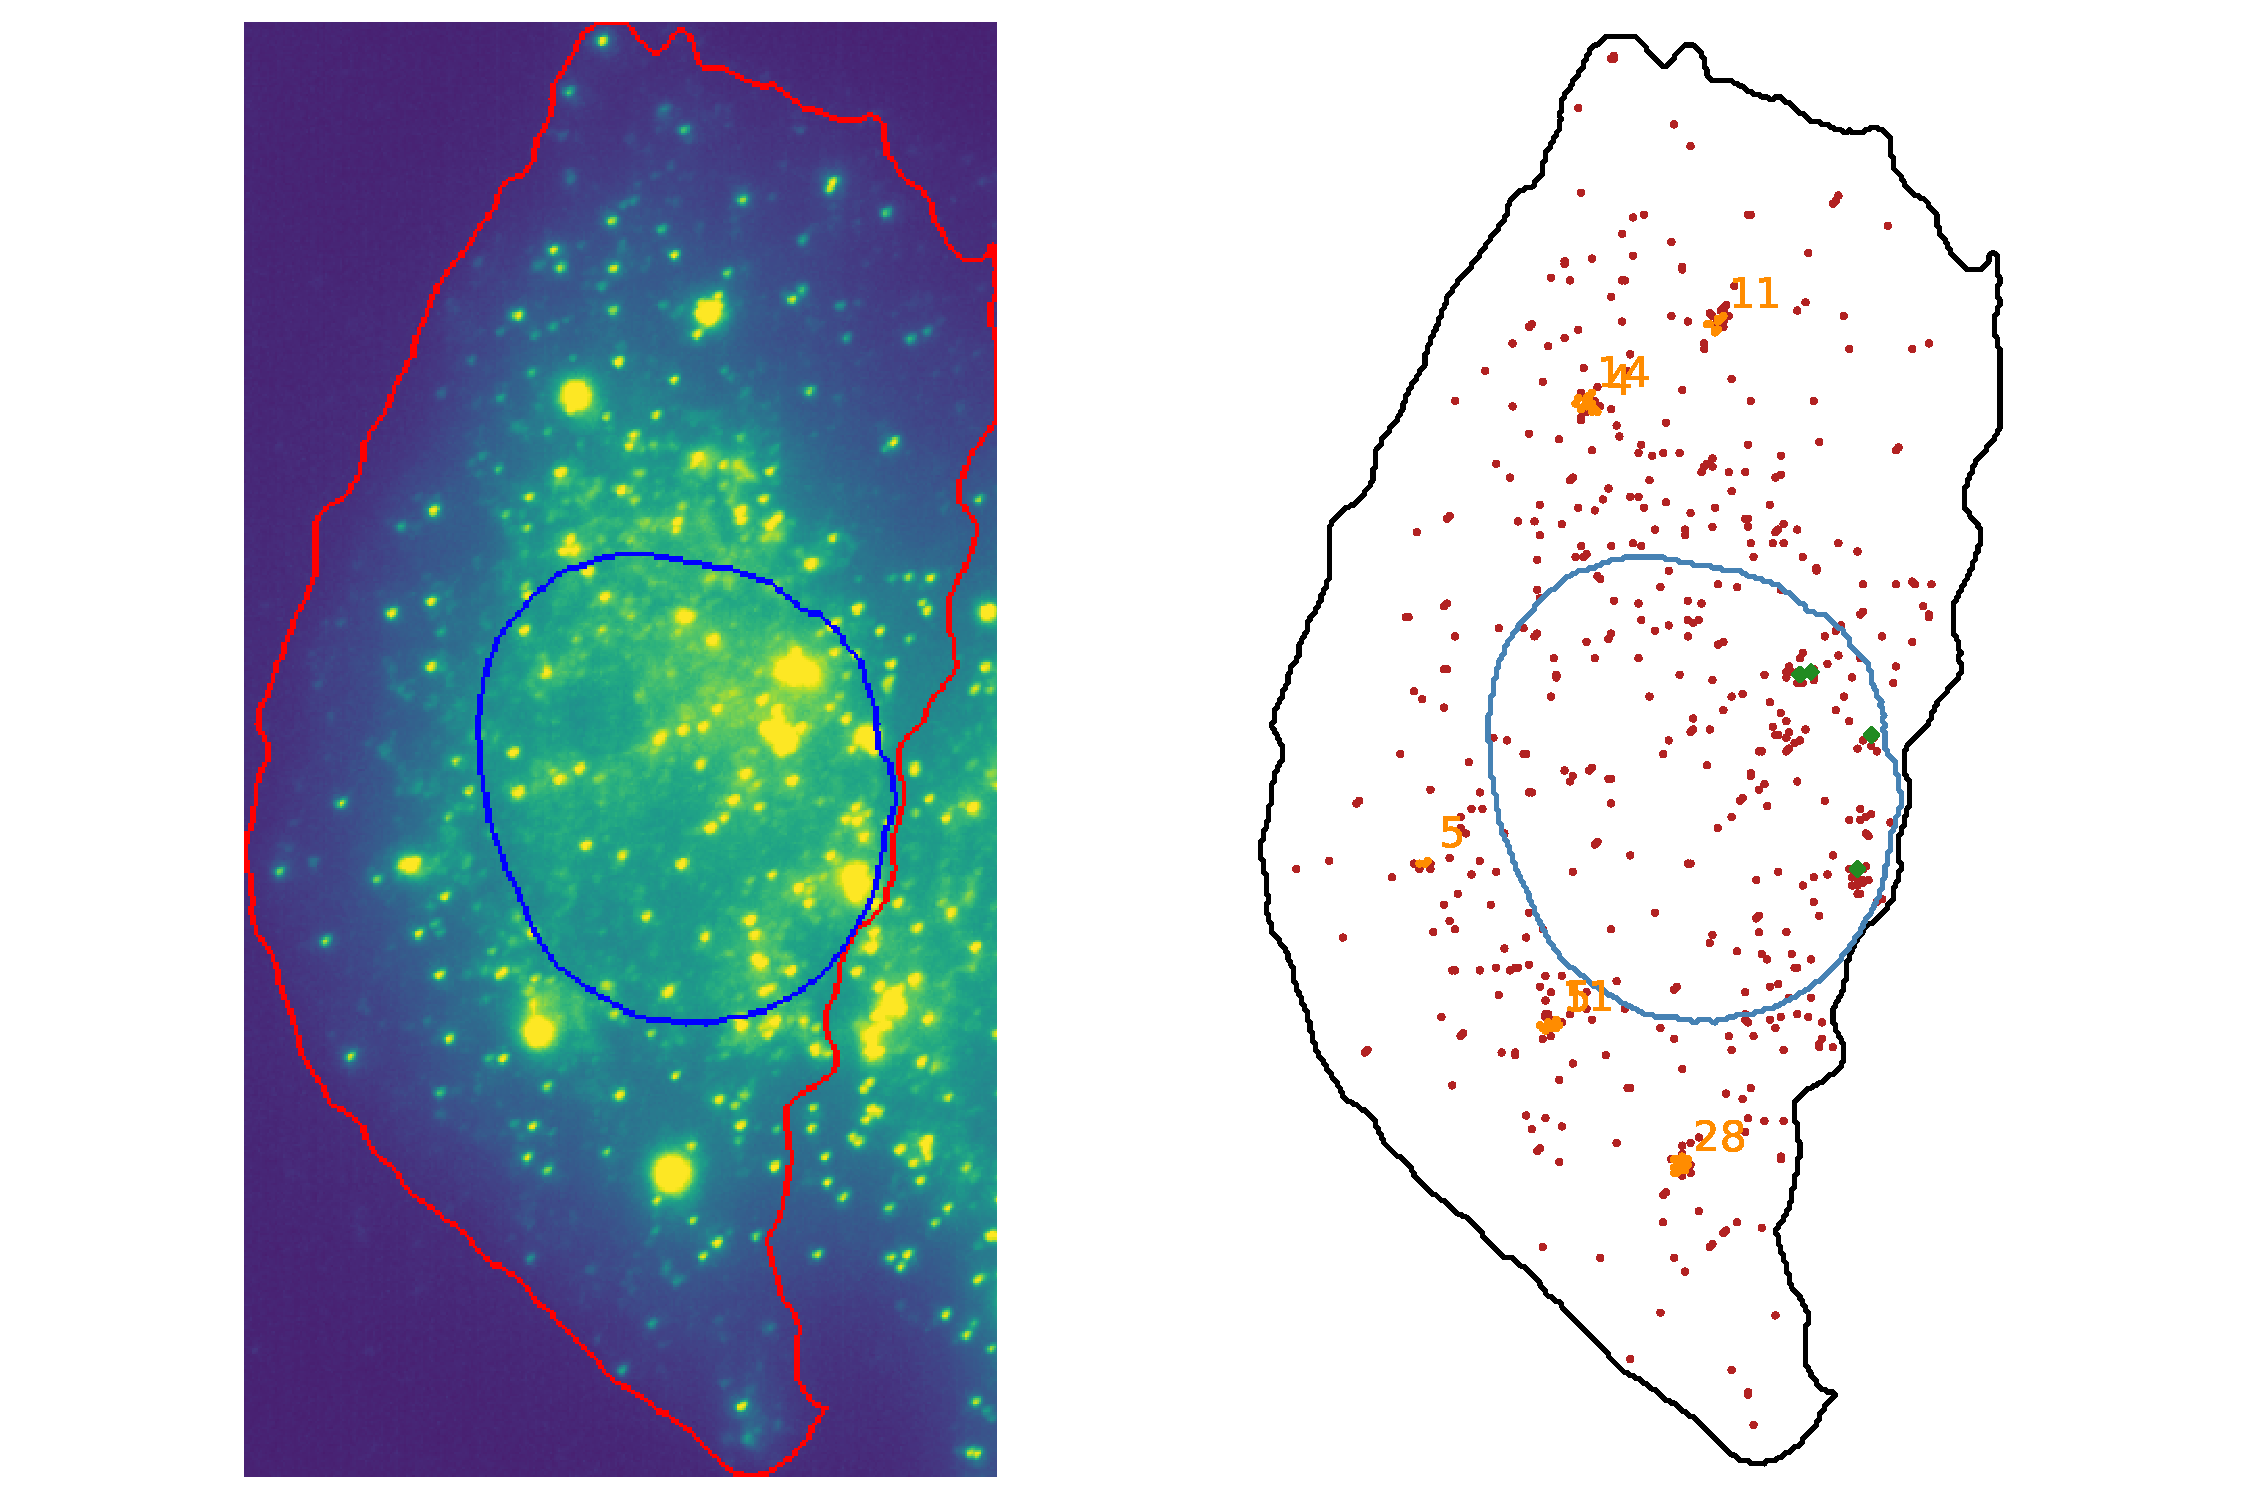
\includegraphics[width=\textwidth]{figures/chapter4/cell_extracted_0}
    \caption[Coordinate representation of a cell]{Contrasted original image with segmented boundaries (\textit{left}) and coordinate representation (\textit{right}).
	Plot build with \emph{bigfish}}
    \label{fig:cell_extracted_0}
\end{figure}

\subsection{Gathering all information at the single cell level}

% a pladoyer for compartmentalization
To extract and summarize \ac{FISH} results at the single cell level, the only requirement is a segmentation mask of the cell, that allows us to associate each detected \ac{RNA} and other objects to one cell. Segmentation of additional compartments is optional, but greatly improves the amount of relevant information on \ac{RNA} localization assigned to each cell. 

\subsubsection{Labeling detected objects according to their localization in the cell}
The nuclei segmentation masks allows us to identify the intra-nuclear RNAs.
Technically, this amounts to assigning a region label to each of the detected RNAs or clusters. In general, the more subcellular compartments are available, the more detailed the description of RNA localization can become in the following

% example of transcription sites vs. other interpretations.
This compartmentalization might also change the interpretation we are giving to detected clusters. For instance, a cluster inside a nucleus might be interpreted as transcription site, while a cluster in the cytoplasm can have various biological interpretations (e.g. P-bodies, translation factories, stress granules). 
In Figure~\ref{fig:cell_extracted_0} we see a cropped \ac{smFISH} image on the left, with cell and nuclear membranes in red and blue respectively.
On the right, these membranes are illustrated in black and blue respectively. 
In addition, we see \ac{RNA} spots (in red), \ac{RNA} clusters (in orange, with the estimated number of \ac{RNA} clustered) and transcription sites (in green). 

In \emph{bigfish} this labeling detected RNAs and clusters can be achieved with a few lines: \\

\begin{minipage}{0.9\textwidth}
\begin{lstlisting}[language=Python]
import bigfish.multistack as multistack

# extract cell-level results
fov_results = multistack.extract_cell(
    cell_label=cell_label,
    ndim=3,
    nuc_label=nuc_label,
    rna_coord=spots_no_ts,
    others_coord={"foci": foci, "transcription_site": ts},
    image=image_contrasted,
    others_image={"dapi": nuc_mip, "smfish": smfish_mip})
\end{lstlisting}
\end{minipage}


% Advantage of this representation
\subsubsection{The advantage of a coordinate representation}
With such \emph{extraction} we lose pixel-wise information like intensity values or image texture.
We also rely on detection and segmentation performances to return meaningful coordinates.
Nonetheless, coordinate representation is a sparse and more natural representation for \ac{mRNA} localization pattern classification: the coordinates - rather than the fluorescence images themselves - represent the actual measurement I want to make, when I perform smFISH experiments. Finally, in contrast to raw images, coordinates of detected objects allow a much more convincing data integration: the number of potential batch effects and biases is greatly reduced. 


\subsubsection{Filtering}
We can also filter the data at the cellular and object level. 
At the cellular level, we might want to ensure that only one nucleus is assigned to each cell, and we can remove cells at the border of the \ac{FoV}. 
Their segmentation is incomplete and might bias final results.
Third, extracted cells can be filtered out according to the number of detected objects (especially the number of \ac{RNA}s).
By censoring empty cells, we remove potential outliers, detection or segmentation failures and therefore help a subsequent statistical analysis.

We can also filter out individual objects according to their localization in the cell. 
A user might want to exclude a detected object if it locates within a segmented surface.
For example, some studies require to remove transcription sites before further analysis~\cite{CHOUAIB_2020}, or on the contrary focus on quantification of transcription sites.\\

\begin{minipage}{0.9\textwidth}
\begin{lstlisting}[language=Python]
import bigfish.multistack as multistack

# discriminate foci and transcription sites
spots_no_ts, foci, ts = multistack.remove_transcription_site(
    rna=spots,
    clusters=clusters,
    nuc_mask=nuc_label,
    ndim=3)
\end{lstlisting}
\end{minipage}

%Individual objects can be discriminated according to their localization in the cell.
% % %A user might want to label a detected object if it locates within a segmented surface or not.
% % For example, some studies require to remove transcription sites before further analysis~\cite{CHOUAIB_2020}, or on the contrary to focus on them.
% % User could define a \ac{RNA} cluster inside the nucleus as a transcription site, as opposed to the ones detected outside nucleus.
% % More generally, any detected object can be assigned to a specific cellular compartments.\\



% Eventually I propose optional criteria to identify individual cells and refine the outcome.
% First, I can ensure that only one nucleus is assigned to each cell.
% Second, I can remove cropped cells at the border of the \ac{FoV}.
% Their segmentation is incomplete and might bias final results.
% Third, extracted cells can be filtered out according to the number of detected objects (especially the number of \ac{RNA}s).
% By censoring empty cells, I remove potential outliers, detection or segmentation failures and therefore help a subsequent statistical analysis.\\



%make us able to delimitate nuclear membrane and define transcription sites or any nucleus-related object.



%Additional results are optional, but they greatly improve the quality of the information assigned to each cell.
%Detected \ac{RNA} and cluster (or anything else detected) can be assigned to individual cells.
%Nuclei segmentation masks make us able to delimitate nuclear membrane and define transcription sites or any nucleus-related object.
%Input images can be also cropped around the identified cells, for every available channel.

% In Figure~\ref{fig:cell_extracted_0} we can observe a cropped \ac{smFISH} image on the left, with cell and nuclear membranes in red and blue respectively.
% On the right, these membranes are also visible (in black and blue respectively), in addition with \ac{RNA} spots (in red), \ac{RNA} clusters (in orange, with the estimated number of \ac{RNA} clustered) and transcription sites (in green).

% With such \emph{extraction} I lose pixel-wise information like intensity values or image texture.
% I also deeply rely on detection and segmentation performances to return meaningful coordinates.
% Nonetheless, coordinate representation is a sparse and more natural representation for \ac{mRNA} localization pattern classification.
% Indeed \ac{mRNA} molecules can be viewed as single point objects distributed in a 3D space.
% Microscopic images with fluorescent labels are here the only medium I have to measure and approximate their localization, but still a medium.
% Ultimately, the original and relevant information is the 3D spatial coordinates of molecules I target.

% Eventually I propose optional criteria to identify individual cells and refine the outcome.
% First, I can ensure that only one nucleus is assigned to each cell.
% Second, I can remove cropped cells at the border of the \ac{FoV}.
% Their segmentation is incomplete and might bias final results.
% Third, extracted cells can be filtered out according to the number of detected objects (especially the number of \ac{RNA}s).
% By censoring empty cells, I remove potential outliers, detection or segmentation failures and therefore help a subsequent statistical analysis.\\



% % Labeling detected objects (such as \ac{RNA} or clusters) according to their cellular compartment provides us with the opportunity to filter out some \ac{RNA} or other detected structures, depending on the scientific question. 
% % %In addition to detection and segmentation refinement, the possibility to merge results from both stages is highly valuable.
% % %Individual objects can be discriminated according to their localization in the cell.
% % %A user might want to label a detected object if it locates within a segmented surface or not.
% % For example, some studies require to remove transcription sites before further analysis~\cite{CHOUAIB_2020}, or on the contrary to focus on them.
% % User could define a \ac{RNA} cluster inside the nucleus as a transcription site, as opposed to the ones detected outside nucleus.
% % More generally, any detected object can be assigned to a specific cellular compartments.\\

% % % reference paper using transcription site only

% % \begin{minipage}{0.9\textwidth}
% % \begin{lstlisting}[language=Python]
% % import bigfish.multistack as multistack

% % # discriminate foci and transcription sites
% % spots_no_ts, foci, ts = multistack.remove_transcription_site(
% % 	rna=spots,
% % 	clusters=clusters,
% % 	nuc_mask=nuc_label,
% % 	ndim=3)
% % \end{lstlisting}
% % \end{minipage}

% \subsection{Coordinate representation}
% \label{subsec:coordinate_representation}

% \subsubsection{Cell extraction}

% \tw{this is entirely unclear ... needs to be rewritten}

% To extract and summarize \ac{FISH} results at the single cell level, the only requirement is a segmentation mask of the cell.
% At least, user needs to perform instance segmentation to be able to identify individual cells.

% Additional results are optional, but they greatly improve the quality of the information assigned to each cell.
% Detected \ac{RNA} and cluster (or anything else detected) can be assigned to individual cells.
% Nuclei segmentation masks make us able to delimitate nuclear membrane and define transcription sites or any nucleus-related object.
% Input images can be also cropped around the identified cells, for every available channel.

% In Figure~\ref{fig:cell_extracted_0} we can observe a cropped \ac{smFISH} image on the left, with cell and nuclear membranes in red and blue respectively.
% On the right, these membranes are also visible (in black and blue respectively), in addition with \ac{RNA} spots (in red), \ac{RNA} clusters (in orange, with the estimated number of \ac{RNA} clustered) and transcription sites (in green).
% With such \emph{extraction} I lose pixel-wise information like intensity values or image texture.
% I also deeply rely on detection and segmentation performances to return meaningful coordinates.
% Nonetheless, coordinate representation is a sparse and more natural representation for \ac{mRNA} localization pattern classification.
% Indeed \ac{mRNA} molecules can be viewed as single point objects distributed in a 3D space.
% Microscopic images with fluorescent labels are here the only medium I have to measure and approximate their localization, but still a medium.
% Ultimately, the original and relevant information is the 3D spatial coordinates of molecules I target.

% Eventually I propose optional criteria to identify individual cells and refine the outcome.
% First, I can ensure that only one nucleus is assigned to each cell.
% Second, I can remove cropped cells at the border of the \ac{FoV}.
% Their segmentation is incomplete and might bias final results.
% Third, extracted cells can be filtered out according to the number of detected objects (especially the number of \ac{RNA}s).
% By censoring empty cells, I remove potential outliers, detection or segmentation failures and therefore help a subsequent statistical analysis.\\


\subsection{Statistical description}

At this stage, standard and useful statistics for every cell can already be computed.
In particular, we can measure cell and nucleus areas, but also \ac{RNA} distribution, inside and outside nucleus.
From cluster coordinates, we can estimate cluster size, as well as proportion of clustered \ac{RNA}s.
\ac{RNA} proportion in specific cellular compartments are also noteworthy.
Such indicators are already relevant to quantify or validate meaningful biological properties.
For example, a recent study~\cite{cochard_rna_2022} uses \emph{bigfish} to estimate \ac{RNA} recruitment in bioengineered condensates (segmented from a \ac{GFP} channel).\\

\begin{minipage}{0.9\textwidth}
\begin{lstlisting}[language=Python]
import bigfish.multistack as multistack

# compute cell-level statistics
df = multistack.summarize_extraction_results(fov_results, ndim=3)
\end{lstlisting}
\end{minipage}

\section{Hand-crafted localization features}
\label{sec:hand_features}

Here I present hand-crafted features I have implemented for the analysis of \ac{RNA} localization patterns. 
In section \ref{subsec:related_work_hand_features}, I present related work. We will see that there is already a large number of features available in the literature. In section \ref{subsec:expert_features}, I present the features I have chosen for our studies. 



\subsection{Related work}
\label{subsec:related_work_hand_features}

\subsubsection{Feature engineering with bioimages}

In bioimage analysis, in particular for High Content Screening, there is an abundant literature on feature families that have been used for cell and whole image classification. They can be roughly categorized into shape features and texture features. Examples include Haralick features~\cite{Haralick1973}, statistical geometric features~\cite{Walker1996}, local binary patterns~\cite{ahonen_2006}, moment based features~\cite{Reeve1992} and morphological granulometries~\cite{Serra1983}, to name a few. 

Such features have been used to classify cells according to their protein localization patterns~\cite{Boland1998, Glory2007}, or their phenotypes~\cite{Wang2008, Jones2009, Walter2010} or classify directly full images with entire cell populations~\cite{Uhlmann2016}. 

Importantly, such feature families are readily available in standard open-source software for computational phenotyping, such as CellProfiler~\cite{Carpenter2006, Jones2008, mcquin_cellprofiler_2018}, CellCognitionn~\cite{held_cellcognition_2010}, Mahotas \cite{mahotas_2013} and ilastik~\cite{berg_ilastik_2019}.  

Most of these hand-crafted features come from the computer vision literature: they are pretty generic with limited biological interpretability. Furthermore, they are designed to quantitatively describe object shapes and textures, rather than directly representing spatial distributions of biomolecules. Of note, this also holds for protein localization screens~\cite{Glory2007, Ouyang2019b}. This is due to the fact that with traditional microscopy, individual proteins cannot be resolved. In addition, proteins can be abundant and often concentrate on specific structures. As a consequence, the protein signal cannot be decomposed into single points, and it is therefore logical to describe their spatial distribution by texture features. A notable exception is provided by super-resolution microscopy, where protein distributions are indeed modeled as point clouds~\cite{Levet2019}. 

In conclusion, there is a need for features describing spatial distributions of RNA molecules inside the cell, implemented in user-friendly open-source tools. 

%existing tools appear limited for a \ac{smFISH} analysis which does not only rely on image texture or cell morphology.

%Features describing the spatial distribution of molecules are therefore still required. 

% Bio-image computing field has long proposed quantitative frameworks and features to explore cellular mechanisms.
% Some popular software includes complete analysis pipelines from image preprocessing to feature engineering.
% For example CellProfiler~\cite{mcquin_cellprofiler_2018} allows researchers to count cell organelles and measure their size, analyze cell shape or extract pixel-wise texture information.
% Expression level computation is also a standard, through proteome quantification.
% CellCognition~\cite{held_cellcognition_2010} proposes a computational framework to annotate and classify relevant biological phenotypes, mostly through morphological measures.
% More than 150 features are available.
% Last but not least, ilastik~\cite{berg_ilastik_2019} also offers classification pipelines, with pixel-wise features such that intensity values, texture, brightness or color gradient.
% Although useful and widely employed, these frameworks appear quickly limited for a \ac{smFISH} analysis which does not only rely on image texture or cell morphology.
% More specialized libraries are needed.

\subsubsection{\ac{RNA} localization features}

Hand-crafted features to classify \ac{RNA} localization patterns were already developed in previous studies~\cite{battich_image-based_2013,samacoits_computational_2018}.
Generally such features are inspired by literature on spatial statistics~\cite{ripley2005spatial} and adapted for fluorescence microscopy images~\cite{lagache_statistical_2015,stueland_rdi_2019}.
Furthermore, several packages implement modules to perform \ac{smFISH} analysis and compute these hand-crafted features~\cite{mueller_fish-quant_2013,savulescu_dypfish_2019,mah_bento_2022}.

In~\cite{battich_image-based_2013}, authors designed 18 features ''that reflect the relative localization of each spot in a single cell, with respect to both the cell and other spots''.
They compute per-transcript features, then exploit their per-cell mean and standard deviation to identify subcellular localization patterns.
They even complete and extend their pipeline analysis in a subsequent work~\cite{stoeger_computer_2015}, by integrating segmentation and detection algorithms.

Two recent Python libraries greatly extend and facilitate the quantification of \ac{FISH} experiments.
DypFISH~\cite{savulescu_dypfish_2019} was developed to analyze \ac{RNA} and protein (co-)localization.
It includes features to investigate clustering and \ac{MTOC}-related patterns.
Across different imaging acquisitions of cells with a architecture constraints, they propose techniques to study \ac{mRNA}-protein spatial distribution~\cite{savulescu_interrogating_2021}.
Bento~\cite{mah_bento_2022} proposes modules to analyze images generated with \ac{SeqFISH} and \ac{MERFISH}.
They adapt feature extraction pipeline to highly multiplexed spatial transcriptomics data.

In FISH-quant v1~\cite{mueller_fish-quant_2013} more than 20 features are implemented in MATLAB.
They are extensively evaluated in a recent publication~\cite{samacoits_computational_2018} with simulated localization patterns.
Compared to previous features developed in the literature~\cite{battich_image-based_2013}, they return a better performance to classify \ac{RNA} localization patterns.
A first set of features includes distance features between \ac{RNA} spots and cell or nucleus.
A second set of features involved the Ripley K-function~\cite{ripley2005spatial}:

\begin{equation}
	{\displaystyle K(r) = \frac{1}{n} \sum_{i = 1}^{n} \frac{N_i(r)}{\lambda}}
\end{equation}

\noindent
With $N_i$ Npi (r) the number of \ac{RNA}s in a circle of radius $r$ centered on the $i^{th}$ \ac{RNA} and $\lambda$ the total density of \ac{RNA}s in the cell.
It quantifies the aggregation or dispersion of mRNAs.
Several features are designed from these values, exploiting their maximum or their correlation with the radius $r$.
However, Ripley features are sensitive to boundary effects (\ac{RNA}s close to a membrane have a limited neighborhood) and require to be correctly normalized.
A third set of features is based on morphological operations, like opening, to identify cell extensions.
Lastly, dispersion and polarization indices are implemented.
Some of my own hand-crafted features are implementations or improvements of this work.

\subsection{Expert features}
\label{subsec:expert_features}

A large part of hand-crafted features I implemented in \emph{bigfish.classification} were initially designed for our own studies~\cite{CHOUAIB_2020,safieddine_choreography_2021,pichon_kinesin_2021}.
These features capture more specific information about \ac{RNA} localization, beyond surface areas (\emph{cell\_area} and \emph{nuc\_area}) or expression levels (\emph{nb\_rna}).

\subsubsection{Distance features}

I first reuse and adapt some distance features already implemented in FISH-quant v1 and presented in a recent paper~\cite{samacoits_computational_2018}.
Distances from cell or nuclear membranes are computed in 2D as I only use 2D segmentation results so far.
However, such features could be easily extended with 3D segmentation masks.
I compute the average distance between detected \ac{RNA}s and cell membrane \emph{index\_mean\_distance\_cell} such that:

\begin{equation}
	{\displaystyle \operatorname{index\_mean\_distance\_cell} = \frac{\overline{d_{cell}(x_i, y_i)}}{\lambda_{cell}}}
\end{equation}

\noindent
With $d_{cell}(x_i, y_i)$ the euclidean distance to the cell membrane for the rna $i$ and $\lambda_{cell}$ the expected average distance under uniform \ac{RNA} distribution.
A previous study~\cite{battich_control_2015} used the square root of cell area to normalize its distance features.
However, as noticed by~\cite{samacoits_computational_2018}, it does not take into account a potential heterogeneity in terms of cell morphology.
For this reason I approximate $\lambda_{cell}$ as the average value of the 2D distance map from the cell membrane.
Similarly, I compute the normalized average distance of \ac{RNA}s to the nucleus: \emph{index\_mean\_distance\_nuc}.
Alternative computation with the median function is available for these two features too.

Unlike FISH-quant v1, I do not compute distances to cell or nucleus centroids, nor quantiles of the \ac{RNA} distance distribution.
These features might appear redundant to quantify distance information.

\subsubsection{Morphological features}

A second set of features is related to the localization of \ac{RNA} in specific cell compartments.
I already count the number of transcripts detected inside the nucleus.
Specifically, the proportion of \ac{RNA}s within the nucleus (\emph{proportion\_rna\_in\_nuc}) is a good enough indicator to identify the intranuclear pattern.

\begin{figure}[]
    \centering
    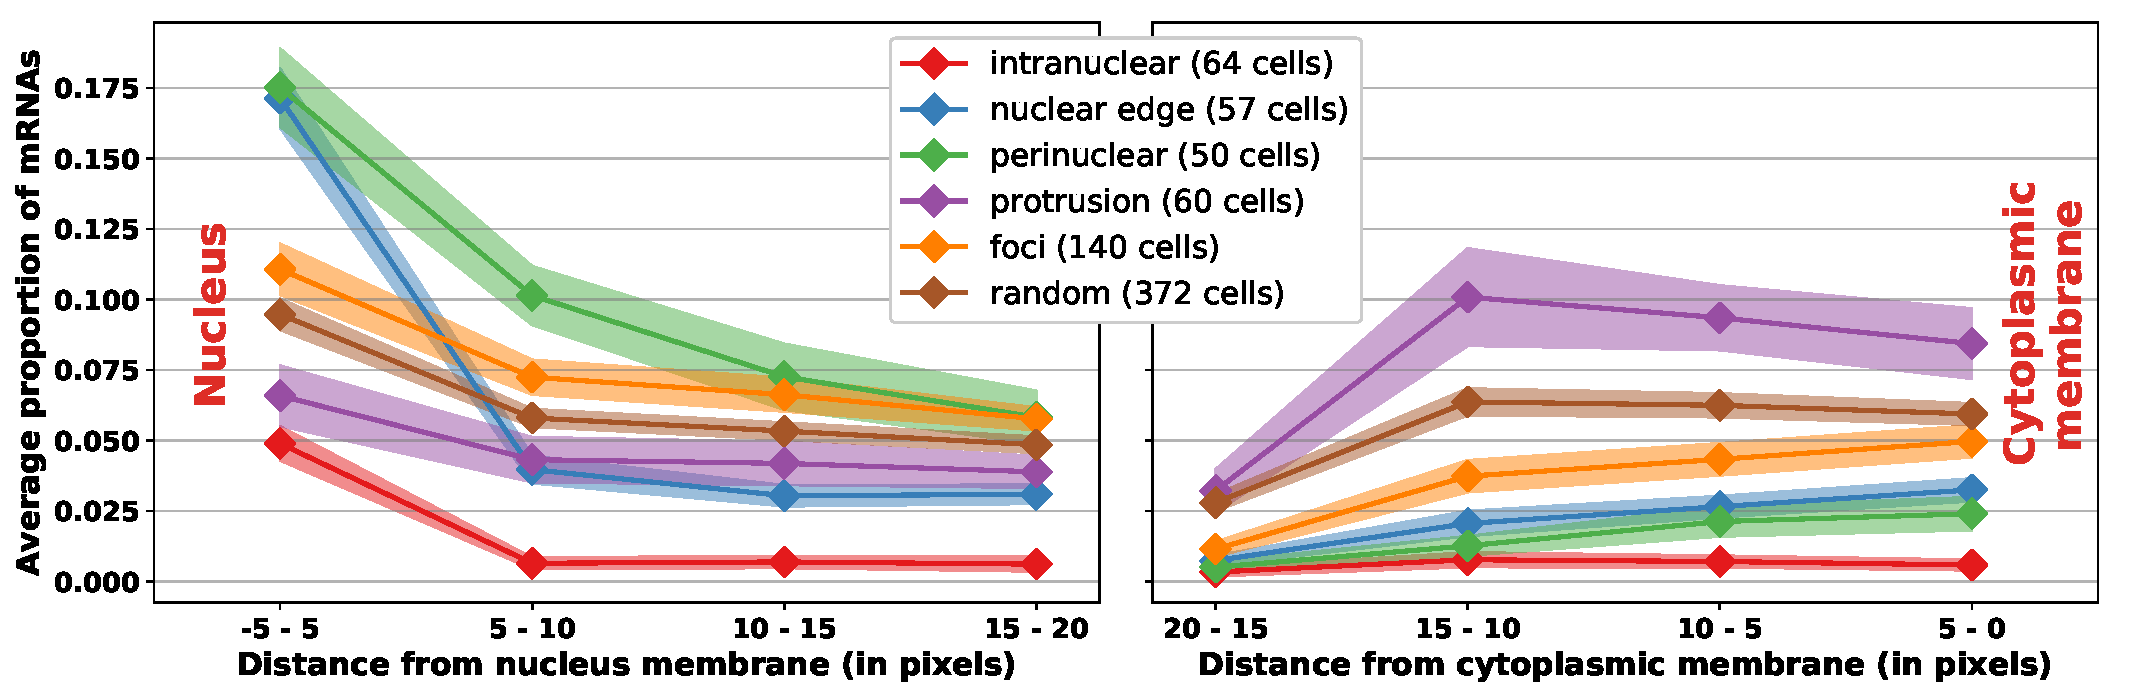
\includegraphics[width=\textwidth]{figures/chapter4/plot_topography}
    \caption[Proportion of mRNAs in several subcellular regions]{Proportion of mRNAs at various distances from cell and nuclear membranes.
	Dataset and annotated patterns from~\cite{CHOUAIB_2020}.
	\textit{Colored areas} represent the 95\% confidence interval}
    \label{fig:features_topography}
\end{figure}

Still I can go further to partition cell regions.
I define a list of features to measure the distribution of \ac{RNA}s within different cell regions.
Regions of interest are delimited with concentric circles from cell or nuclear membranes, with an interval distance of 500nm each.
More precisely, area between 0 and 3000nm from the cell membrane is divided in six concentric regions.
In each region I compute \ac{RNA} proportion (\emph{proportion\_rna\_cell\_radius\_1000\_1500} for the proportion between 1000nm and 1500nm from the cell membrane) or I count the number of \ac{RNA}s I detect, normalized by the expected number of \ac{RNA}s under random distribution (\emph{index\_rna\_cell\_radius\_1000\_1500}).
I also define 5 more regions around the nuclear membrane between 500nm and 3000nm.
Another region is defined along the nuclear membrane, including detected \ac{RNA}s inside or outside the nucleus, but within 500nm from its membrane.
Likewise, proportion (\emph{proportion\_rna\_nuc\_radius\_500\_1000}) and normalized \ac{RNA} count (\emph{index\_rna\_nuc\_radius\_500\_1000}) are computed for all regions around the nuclear membrane.
When I manually annotate real cells and identify different localization pattern I can measure how discriminative these features can be.
In Figure~\ref{fig:features_topography} we observe average \ac{RNA} proportion for the different regions I described.
The 95\% confidence interval is also reported in the plot.
Logically, nuclear edge and perinuclear patterns present a higher proportion of \ac{RNA}s along the nuclear membrane.
On the opposite, cells with a protrusion pattern have a higher \ac{RNA} density along the cell membrane.

I focus on a last relevant region in a cell: protrusions.
To design features related to cell extension I first need to define such extension.
Like~\cite{samacoits_computational_2018} I define this region as the lost area after applying a morphological opening (an erosion followed by a dilation) to the cell mask.
For this operation I use a disk with 3000nm radius as a structuring element.
I then compute the proportion of \ac{RNA}s (\emph{proportion\_rna\_protrusion}) or the normalized \ac{RNA} count (\emph{index\_rna\_protrusion}) in protrusion.

\subsubsection{Dispersion features}

I implement three features described and tested in a recent paper~\cite{stueland_rdi_2019} to quantify \ac{RNA} polarization and dispersion within the cell.

Polarization index is computed by comparing \ac{RNA} point cloud centroid and cell centroid:

\begin{equation}
	{\displaystyle \operatorname{index\_polarization} = \frac{\sqrt{(x_{rna} - x_{cell})^2 + (y_{rna} - y_{cell})^2}}{Rg_{cell}}}
\end{equation}

\noindent
With $(x_{rna}, y_{rna})$ the coordinates of the \ac{RNA} centroid and $(x_{cell}, y_{cell})$ the coordinates of the cell centroid.
The radius of gyration $Rg_{cell}$ normalizes the index for different cell sizes.
It is defined as the root-mean-squared distance between every cell pixel and the cell centroid.
The higher, the more polarized \ac{RNA}s are.

Dispersion index measures the dispersion of the \ac{RNA} point cloud.
In addition to the extracted coordinates, its computation also implies pixel intensities from the original \ac{smFISH} image:

\begin{equation}
	{\displaystyle \operatorname{index\_dispersion} = \frac{\frac{\sum_{i} r_i^2 I_i}{\sum_{i} I_i}}{\frac{\sum_{j} r_j^2 I_j}{\sum_{j} I_j}}}
\end{equation}

\noindent
With $r_i$ and $r_j$ the euclidean distance of \ac{RNA} $i$ and cell pixel $j$ to the \ac{RNA} centroid respectively, $I_i$ the pixel intensity of \ac{RNA} $i$ and $I_j$ the pixel intensity of cell pixel $j$.
Pixel intensity of transcripts distant from the \ac{RNA} centroid are overweighted.
As the index is normalized considering every pixel $j$ from the cell mask, it tends to 1 when \ac{RNA} point cloud is uniformly distributed.
A diffuse point cloud has a value greater than 1.
On the opposite, if \ac{RNA}s are concentrated anywhere in the cell, index value is lower than 1.

Peripheral distribution index measures how close the \ac{RNA}s localize to the cell periphery (\emph{index\_peripheral\_distribution}).
Its computation is similar to the dispersion index, but the \ac{RNA} centroid is replaced by the nucleus centroid in the equation.
A completely dispersed point cloud still has a value of 1, but it increases if \ac{RNA}s move toward the cell periphery, with a concentrated or diffused pattern.
Again, an aggregation of transcripts around the nucleus centroid (often close to the cell centroid too) decreases index value.

\subsubsection{Centrosomal features}

\begin{wrapfigure}{R}{0.40\textwidth}
	\begin{center}
	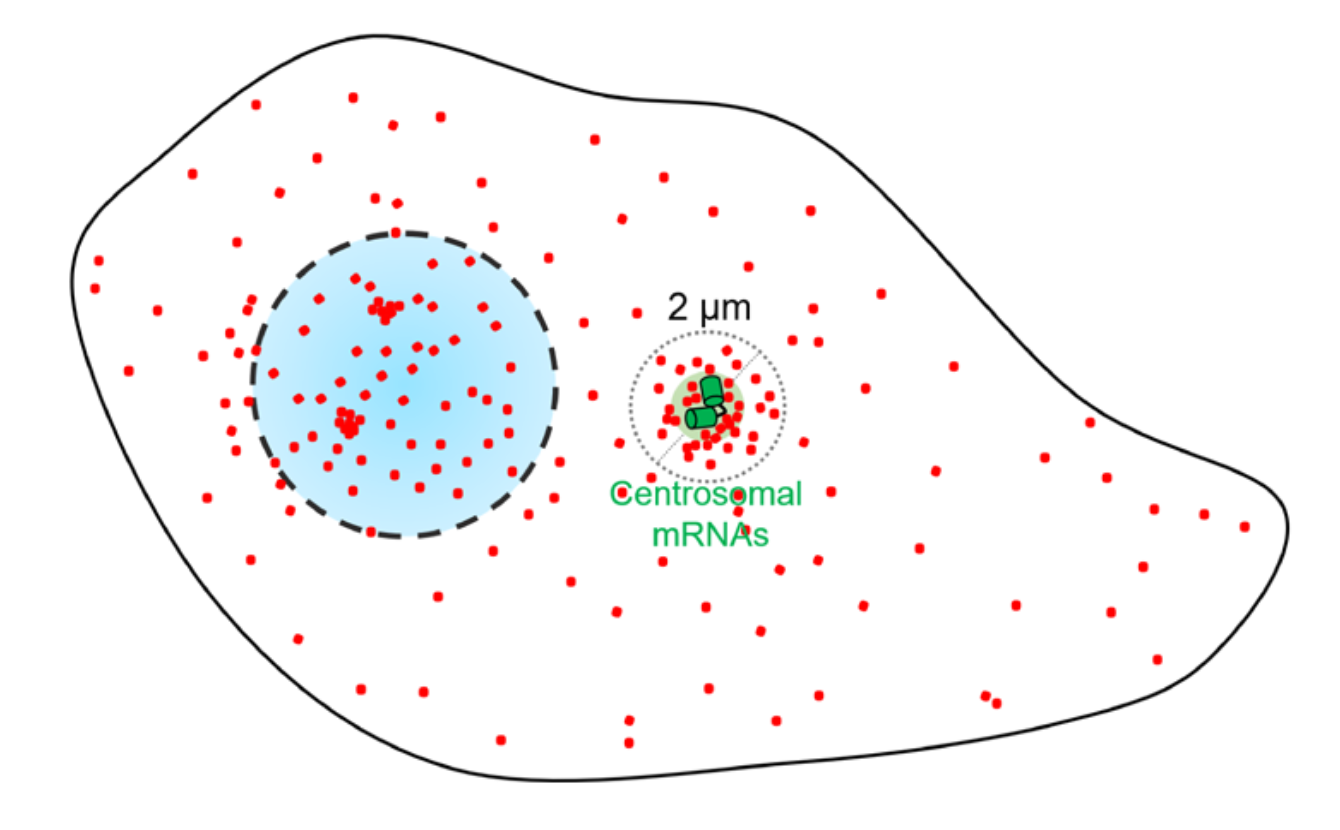
\includegraphics[width=\linewidth]{figures/chapter4/centrosomal_features}
	\caption[Centrosomal neighborhood]{Centrosomal RNAs and its neighborhood from~\cite{safieddine_choreography_2021}}
	\label{fig:centrosome_features}
	\end{center}
\end{wrapfigure}

If I detect additional object and extract new coordinates besides individual and clustered \ac{RNA}s, more specific features can be designed.
For example, these objects can be cell organelles labelled during the experimentation.
I design such features with the centrosomes to further study \ac{RNA} localization related to the \ac{MTOC}~\cite{safieddine_choreography_2021}.

A first obvious feature is the average (or median) distance between \ac{RNA}s and the closest detected centrosomes (up to two centrosomes can be detected in the cell): \emph{index\_mean\_distance\_centrosome}.
Similarly to the distance features I compute with the cell or nuclear membranes, I compute the expected distance under uniform \ac{RNA} distribution for normalization.

A second set of features consists in delimiting an area around each centrosome to be considered as centrosome's neighborhood.
In my case I manually choose a radius of 2000nm around centrosomes to define such areas, as illustrated in Figure~\ref{fig:centrosome_features}.
I can then compute normalized \ac{RNA} count (\emph{index\_rna\_centrosome}) or \ac{RNA} proportion (\emph{proportion\_rna\_centrosome}) in these regions.

Lastly, I derived a feature from the dispersion index described above.
I define a centrosomal dispersion index to quantify \ac{RNA} dispersion around centrosomes: \emph{index\_centrosome\_dispersion}.
I design it like the dispersion index, but instead of \ac{RNA} centroid, I use the closest centrosome coordinates to compute the euclidean distance.
The lower, the closer \ac{RNA}s localized to the centrosomes.

\subsubsection{Cluster features}

Concerning cluster localization patterns, I observed that my clustering method (see subsection~\ref{subsec:dense_decomposition}) already captures good enough information.
More specifically, number of detected clusters (\emph{nb\_foci}) or \ac{RNA} proportion inside these clusters (\emph{proportion\_rna\_in\_foci}) are relevant features to identify transcripts with a tendency for clustering.
As a consequence, and unlike~\cite{samacoits_computational_2018}, I do not implement diverse features based on the famous Ripley's K-function.
This would require tuning a lot more parameters than just reusing the detected number of clusters.\\

\begin{minipage}{0.9\textwidth}
\begin{lstlisting}[language=Python]
import bigfish.classification as classification

# compute features
features, features_names = classification.compute_features(
    cell_mask=cell_mask,  # individual cell mask
	nuc_mask=nuc_mask,  # individual nucleus mask
	ndim=3,
	rna_coord=rna_coord,
    smfish=smfish,
	voxel_size_yx=103,  # in nanometer
    foci_coord=foci_coord,
    compute_distance=True,
    compute_intranuclear=True,
    compute_protrusion=True,
    compute_dispersion=True,
    compute_topography=True,
    compute_foci=True,
    compute_area=True,
    return_names=True)
\end{lstlisting}
\end{minipage}

\section{Learned localization features}
\label{sec:learned_features}

A second approach to analyze \ac{RNA} localization patterns is to learn features.
To this end I design and train a deep learning model, PointFISH, on a simulated pretext task~\cite{pointfish_2022}.
I then reuse the internal representation learned by the model as a point cloud embedding to discriminate \ac{RNA} localization patterns.
The later is evaluated on an experimental dataset.

\subsection{Related work}
\label{subsec:related_work_learned_features}

\subsubsection{Learning features and embeddings}

A neural network learns representations that I can use for transfer learning.
One advantage is to pretrained relevant representations on a first task with a large and general annotated dataset, before addressing a more difficult or specific task with sometimes a limited dataset available.
Such model can be used as a feature extractor by computing features from one of its intermediate layers.
Computer vision community progressively replaces hand-crafted features~\cite{Lowe_1999,Bay_2006} by deep learning features to analyze images.
Best convolutional neural networks pretrained on large and general classification challenges~\cite{He_2016_CVPR,Szegedy_2016_CVPR,Tan_2019,Huang_2017_CVPR} are used as backbone or feature extractor for more complex task like face recognition, detection or segmentation.
NLP community follows this trend as well with a heavy use of word embeddings~\cite{Mikolov_2013,Joulin_2016} or the more recent transformers models.
As a last example, with graph computation, node2vec~\cite{Grover_2016} learns ''task-independent representations'' for nodes in networks.

Such embedding has also the advantage to be a continuous and numerical representation.
This is especially useful when dealing with a non-structured data like text or graph.
With spage2vec~\cite{Partel_2021}, authors learn a low dimensional embedding of local spatial gene expression (expressed as graphs).
Eventually, they identify meaningful gene expression signatures by computing this embedding for tissue datasets.

\subsubsection{Convolutional features}

Because I analyze smFISH images, a first intuition would be to build a convolutional neural network to directly classify localization patterns from the fluorescent image.
This approach is actually already in place for protein localization.
Unlike RNA, proteins are usually studied with fluorescent protein, like \ac{GFP} markers, and are difficult to resolve individually.
In this case, they appear as a gradient of intensity in the fluorescent image and thus protein localization has often been approached like texture classification problem.
First studies~\cite{boland_automated_1998} for example compute a set of feature from the microscopy image before training a classifier.
With recent successes of deep learning, protein localization is now tackled with convolutional neural network, but still framed as a texture classification problem.
After crowdsourcing annotations for the Human Protein Atlas dataset~\cite{Uhlen_2015} (through a video game), researchers trained a machine learning model (Loc-CAT) from hand-crafted features to predict subcellular localization patterns of proteins~\cite{sullivan_deep_2018}.
In a second time, they organized an online challenge~\cite{ouyang_analysis_2019} where a majority of top-ranking solutions were based on convolutional neural networks.
For protein localization the shift from hand-crafted features to convolutional features is significant and allows more accurate and robust pipelines.

A recent perspective paper~\cite{Savulescu_2021} fosters the use of deep learning models for RNA localization analysis.
Today, such analysis can be performed with fluorescent images or RNA sequencing.
Authors emphasize the recent successes and flexibility of neural nets with both types of input, and therefore the possibility to design a multimodal pipeline.
However, smFISH images have clear spots that can be individually resolved and easily detected.
Therefore, a texture classification approach seems suboptimal to address \ac{RNA} localization pattern recognition.

% references CNN for biological images
% Moen, E. et al. Deep learning for cellular image analysis. Nat. Methods https://doi.org/10.1038/s41592-019-0403-1 (2019).
% Godinez, W. J., Hossain, I., Lazic, S. E., Davies, J. W. & Zhang, X. A multi-scale convolutional neural network for phenotyping high-content cellular images. Bioinforma. Oxf. Engl. 33, 2010–2019 (2017).
% Hofmarcher, M., Rumetshofer, E., Clevert, D.-A., Hochreiter, S. & Klambauer, G. accurate prediction of biological assays with high-throughput microscopy images and convolutional networks. J. Chem. Inf. Model. 59, 1163–1171 (2019).
% Kraus, O. Z., Ba, J. L. & Frey, B. J. Classifying and segmenting microscopy images with deep multiple instance learning. Bioinformatics 32, i52–i59 (2016).

\subsubsection{Point cloud models}

I postulate that learning to classify RNA localization patterns directly from detected spots coordinates is the most efficient approach.
A point cloud has an unordered and irregular structure.
Projecting the coordinates into images or voxels~\cite{Maturana_2015} transforms the problem as an easier vision challenge, but it comes along with some input degradations.
It dramatically increases the memory needed to process the sample and loses relevant spatial information.
In case of \ac{RNA} point cloud, I have already explored this approach by using convolutional neural network on a binary image of the point cloud~\cite{dubois_deep_2019}.
It makes the recognition of 3D localization patterns harder~\cite{dubois_deep_2019}.
A more detailed description of the method is available in appendix~\ref{ch:convolutional_features}.

A recent paper~\cite{khater_caveolae_2019} proposes to train a machine learning pipeline to discriminate caveolae clusters from scaffolds clusters.
These cell structures can be recognized through the detection of caveolin-1 proteins and the shape of the resulting point clouds acquired from \ac{SMLM} techniques.
Authors compare three pipelines to address the problem: a random forest classifier trained on hand-crafted features, a convolutional neural network applied on the point cloud image and more importantly a PointNet fed directly with point cloud.
Albeit legitimate, the PointNet method is less successful for this task than the two others pipelines.
Possibly, this model is too naive.

PointNet~\cite{Qi_2017_CVPR} is a seminal work that leads the way for innovative models to address shape classification.
It directly processes point clouds with share MLPs and a max pooling layer, making the network invariant to input permutation.
However, the pooling step is the only way for the model to share information between close points, which ultimately limits its performance.
Yet, recent research dramatically improves point cloud modelling and especially the capture of local information.

PointNet++~\cite{Qi_2017} learns local geometric structures by recursively applying PointNet to different regions of the point cloud, in a hierarchical manner.
This way, local information can be conveyed through the network more efficiently.
DGCNN~\cite{Wang_2019} proposes a new EdgeConv layer where edge features are computed between a point and its neighbors.
Some models propose to adapt convolutions to point cloud by designing new weighting functions or kernel operations like PointCNN~\cite{Li_2018}, PointConv~\cite{Wu_2019_CVPR} or KPConv~\cite{Thomas_2019_ICCV}.
Another inspiration from the computer vision or NLP literature is the attention-based model.
To this end, PointTransformer~\cite{Zhao_2021_ICCV} proposes an attention layer to be applied to local regions within the point cloud.
Last but not least, PointMLP~\cite{ma2022rethinking} proposes a simple but still efficient network with a pure deep hierarchical MLP architecture.

\subsection{Problem statement}
\label{subsec:problem_statement}

I want to train a model, where I can provide directly the point cloud coordinates as an input and compute a continuous vector representation.
This representation can then be used for classification of different \ac{RNA} localization patterns.
Such a deep learning model might require a large volume of annotated data to reach a satisfying performance.
To generate such a large data sets, I used simulated data to train my point cloud model and then use it as a trained feature extractor.
Eventually I evaluate these learned features on a experimental dataset.

\begin{figure}[]
	\centering
	\minipage{0.33\textwidth}
		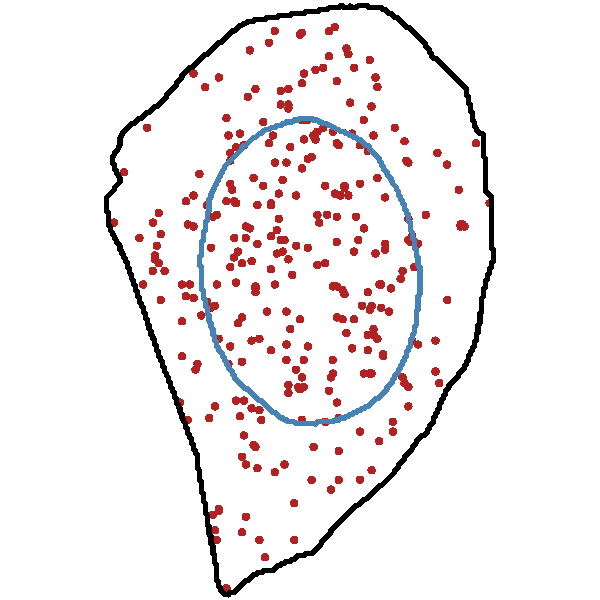
\includegraphics[width=\linewidth]{figures/chapter4/simulation_foci_10}
		\subcaption{10\% clustered RNA}
	\endminipage\hfill
	\minipage{0.33\textwidth}
		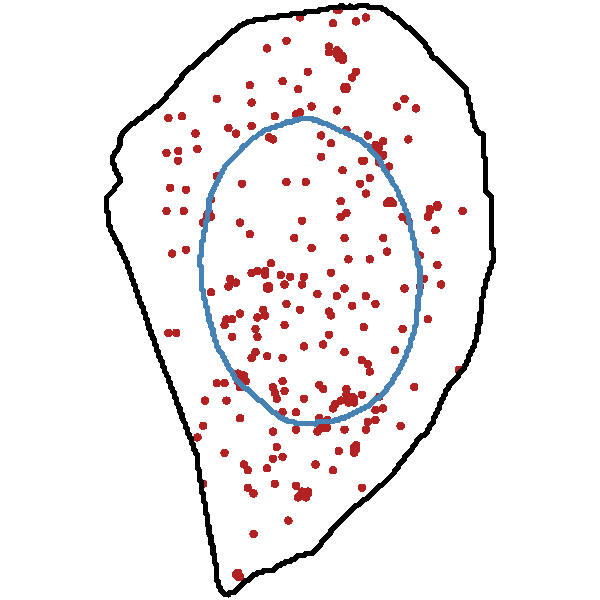
\includegraphics[width=\linewidth]{figures/chapter4/simulation_foci_50}
		\subcaption{50\% clustered RNA}
	\endminipage\hfill
	\minipage{0.33\textwidth}
		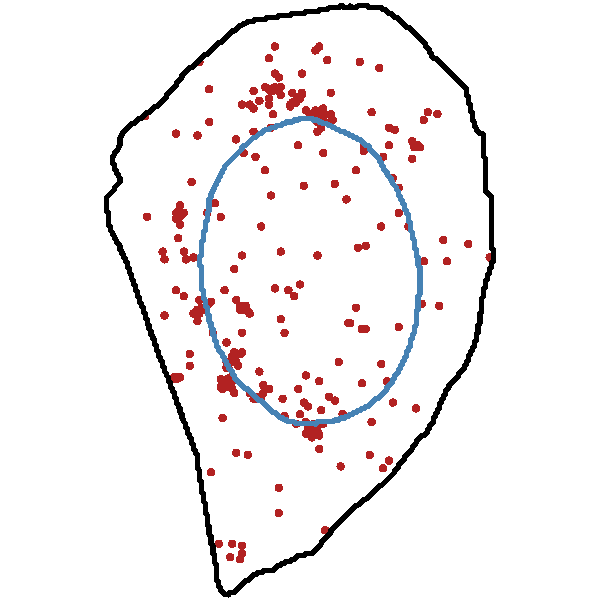
\includegraphics[width=\linewidth]{figures/chapter4/simulation_foci_90}
		\subcaption{90\% clustered RNA}
	\endminipage
	\caption[Simulated foci patterns]{Foci pattern with increasing pattern strength simulated with \emph{simfish}}
	\label{fig:foci_panel}
\end{figure}

\subsubsection{Localization pattern simulations}

To build my simulated dataset, I use methods implemented in \emph{simfish}.
My package exploits a template of 318 real cells to simulate realistic point clouds.
They were originally extracted for FISH-quant v1~\cite{samacoits_computational_2018} to simulate realistic cell and nucleus shapes.
I have the 3D segmentation masks for the cell and the nucleus.
In addition, I have manual annotations about potential protrusions, in case I want to simulate this specific pattern.
Several improvements are brought by \emph{simfish}:
\begin{itemize}
	\setlength\itemsep{0.1em}
	\item I migrate to Python and do not rely on a proprietary framework anymore.
	\item I accelerate the simulation process.
	\item I extend the number of localization patterns available.
	\item I make simulations more consistent in terms of pattern strength.
\end{itemize}

Simulation's outcome includes the cell mask and its membrane coordinates (in 2D), the nucleus mask and its membrane coordinates (in 2D) and the \ac{RNA} coordinates (in 3D).
To match with the rest of the \emph{bigfish} pipeline, I voluntarily return 2D membrane coordinates.
A first parameter to set is the number of \ac{RNA}s $n$ I want to simulate.
To modulate the pattern strength, I set the proportion of \ac{RNA}s $p$ with a biased localization I want.
For example to simulate pattern with a moderate strength, I can simulate between 30\% and 50\% of the \ac{RNA} with the targeted localization bias, and the rest uniformly across the cell.
Lastly, I choose a pattern to simulate.

\begin{figure}[]
	\centering
	\minipage{0.33\textwidth}
		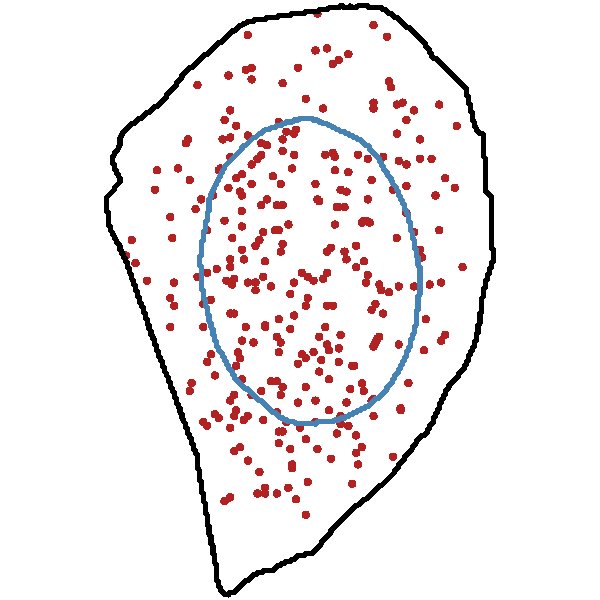
\includegraphics[width=\linewidth]{figures/chapter4/simulation_perinuclear_10}
		\subcaption{10\% perinuclear RNA}
	\endminipage\hfill
	\minipage{0.33\textwidth}
		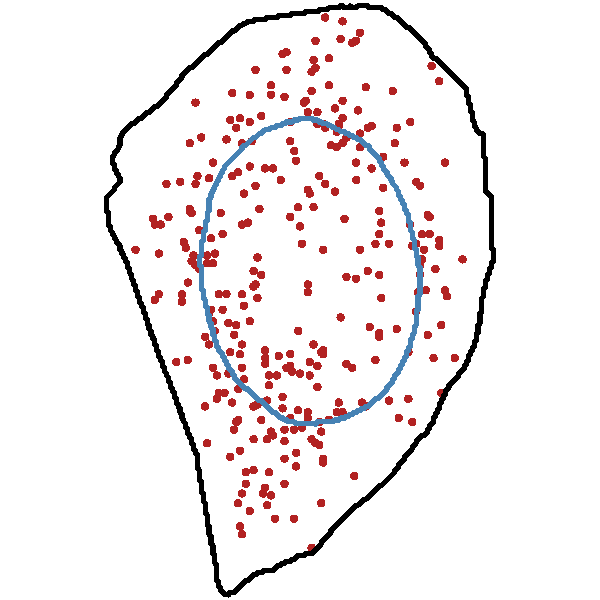
\includegraphics[width=\linewidth]{figures/chapter4/simulation_perinuclear_50}
		\subcaption{50\% perinuclear RNA}
	\endminipage\hfill
	\minipage{0.33\textwidth}
		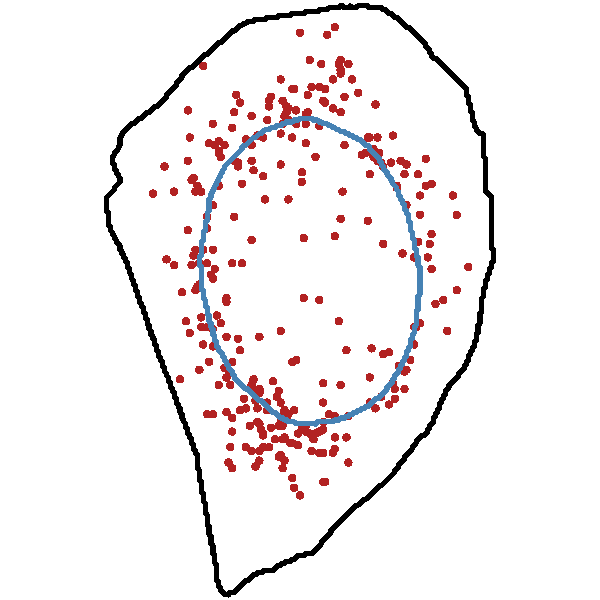
\includegraphics[width=\linewidth]{figures/chapter4/simulation_perinuclear_90}
		\subcaption{90\% perinuclear RNA}
	\endminipage
	\caption[Simulated perinuclear patterns]{Perinuclear pattern with increasing pattern strength simulated with \emph{simfish}, from~\cite{pointfish_2022}}
	\label{fig:perinuclear_panel}
\end{figure}

The 9 patterns currently available are: random, foci, intranuclear, extranuclear, nuclear edge, perinuclear, cell edge, pericellular and protrusion.
Random pattern is the default pattern where \ac{RNA}s are simulated uniformly within the cell.
Foci pattern consists in a random number of \ac{RNA} clusters localizing outside the nucleus.
More precisely, I compute the total number of clustered \ac{RNA}s as $n_{pattern} = n \times p$.
I draw the expected number of \ac{RNA}s $\lambda$ per cluster from a uniform distribution between 5 and 21 \ac{RNA}s.
The number of clusters itself results from $n_{cluster}= \frac{n_{pattern}}{\lambda}$.
For each cluster, a distinct number of \ac{RNA}s is drawn again with a Poisson distribution of mean $\lambda$.
Clusters are then localized outside the nucleus and remaining \ac{RNA}s uniformly in the cell.
In Figure~\ref{fig:foci_panel} we can observe foci simulations with an increasing pattern strength (from 10\% to 90\% of clustered \ac{RNA}s)

Other patterns are simulated with a common scheme.
In a first step I generate a probability map to bias the localization of $n_{pattern}$ \ac{RNA}s.
In a second step I complete the point cloud with random \ac{RNA}s until I reach the expected number of transcripts.
Intranuclear pattern has a uniform probability map inside the nucleus and zeros outside.
Extranuclear pattern is the exact opposite, with nonzero probabilities outside the nucleus and zero inside.
Nuclear edge and cell edge have nonzero probabilities along the nuclear and cell membranes.
Similarly, perinuclear and pericellular are patterns where \ac{RNA}s are polarized towards nuclear and cell membranes.
Perinuclear probability map is build from the cell distance map.
I contrast the euclidean distance by computing its quadratic values.
The same operation is performed to build the pericellular probability map, using the nucleus distance map.
As a result, for pericellular pattern, \ac{RNA}s have a higher probability to localize in regions distant from nucleus.
Protrusion pattern has a uniform probability map within the annotated protrusion regions and zeros everywhere else.
In Figure~\ref{fig:perinuclear_panel} different perinuclear simulations can be observed as an example.
In addition, an overview of every simulated pattern is available in appendix~\ref{sec:appendix_simulations_pattern}.\\

\begin{minipage}{0.9\textwidth}
\begin{lstlisting}[language=Python]
import simfish as sim

# load template dataset
path_template_directory = load_extract_template(path_output)

# localization pattern simulation
instance_coord = sim.simulate_localization_pattern(
	path_template_directory,
	n_spots=150,
	pattern="intranuclear",
	proportion_pattern=0.6)
\end{lstlisting}
\end{minipage}

\subsubsection{Simulated dataset}

\begin{wraptable}{R}{0.50\textwidth}
	\centering
	\begin{tabular}{| c | c |}
		\hline
		Pattern & \# of cells \\
		\hline
		Random & 372\\
		Foci & 198\\
		Intranuclear & 73\\
		Nuclear edge & 87\\
		Perinuclear & 64\\
		Protrusion & 83\\
		\hline
	\end{tabular}
	\caption[Annotated experimental dataset for RNA localization patterns]{Annotated experimental dataset}
	\label{table:real_dataset}
\end{wraptable}

With \emph{simfish} I simulate a dataset with 8 different localization patterns: random, foci, intranuclear, extranuclear, nuclear edge, perinuclear, cell edge and pericellular.
I choose these patterns since they represent a diverse panel of localization patterns in different subcellular regions.
I simulate for each pattern 20,000 cells with 50 to 900 \ac{RNA}s per cell, resulting in a full dataset of 160,000 simulated cells.
Random pattern excepted, every simulated pattern has a proportion of \ac{RNA}s with preferential localization ranging from 60\% to 100\%.
With random simulations the pattern strength has no effect.
I split my dataset between train, validation and test, with 60\%, 20\% and 20\% respectively.
In order to avoid data leakage, I make sure that simulations from the same cell template cannot be assigned to different splits.
Finally, point clouds are augmented with random rotation along the up-axis, centered and normalized into the unit sphere.
In order to test how my trained features generalize to unknown localization patterns, I did not simulate \ac{RNA} localization in protrusions, while these localization class is present in the experimental dataset.
It also prevent my model from training on a too specific pattern.

\subsubsection{Experimental dataset}

I use the experimental dataset extracted from our study~\cite{CHOUAIB_2020} to validate the feature representation learned on simulated images.
Images are obtained from a \ac{smFISH} study in HeLa cells targeting 27 different genes, then processed with \emph{bigfish}.
After cleaning, it consists of 9710 individual cells, with cropped images and coordinates extracted.
Cells have on average 346 \ac{RNA}s in average and 90\% of them have between 39 and 1307 transcripts.
Furthermore, 810 cells have manually annotated localization patterns, as detailed in Table~\ref{table:real_dataset} and illustrated in Figure~\ref{fig:localization_patterns_racha_features}.
Importantly, these patterns are not mutually exclusive since cells can display several patterns at the same time (for example foci with a perinuclear distribution).
I use these annotations as a ground truth for validation.

\begin{figure}[]
	\centering
	\minipage{0.2\textwidth}
		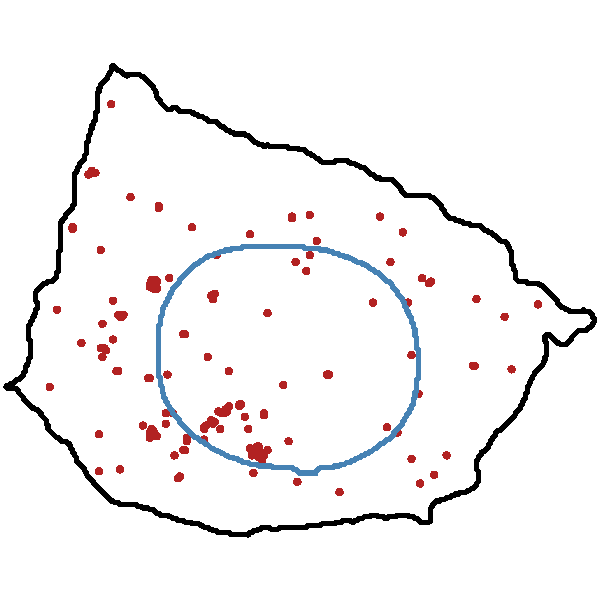
\includegraphics[width=\linewidth]{figures/introduction/real_coord_foci}
		\subcaption{Foci}
	\endminipage\hfill
	\minipage{0.2\textwidth}
		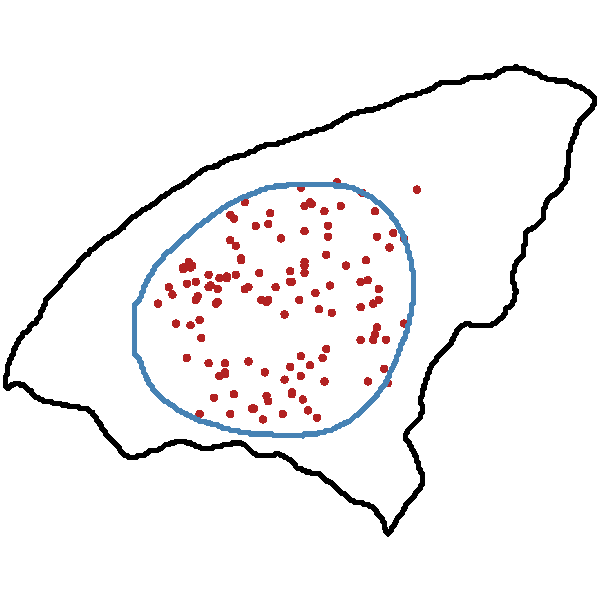
\includegraphics[width=\linewidth]{figures/introduction/real_coord_intranuclear}
		\subcaption{Intranuclear}
	\endminipage\hfill
	\minipage{0.2\textwidth}
		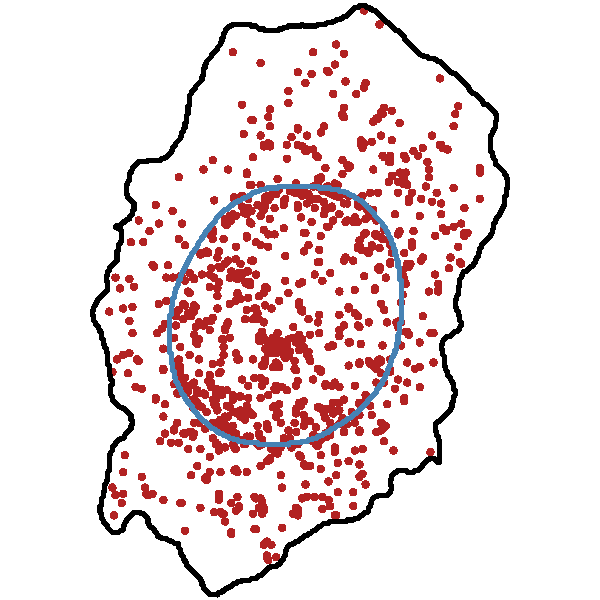
\includegraphics[width=\linewidth]{figures/introduction/real_coord_nuclear_edge}
		\subcaption{Nuclear edge}
	\endminipage\hfill
	\minipage{0.2\textwidth}
		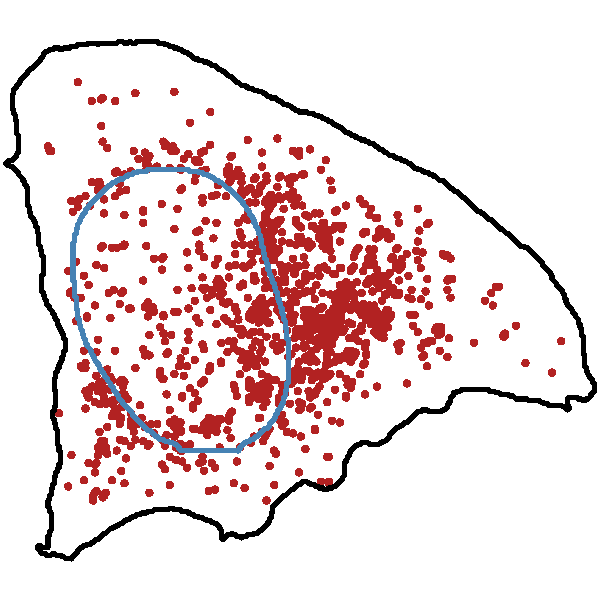
\includegraphics[width=\linewidth]{figures/introduction/real_coord_perinuclear}
		\subcaption{Perinuclear}
	\endminipage\hfill
	\minipage{0.2\textwidth}
		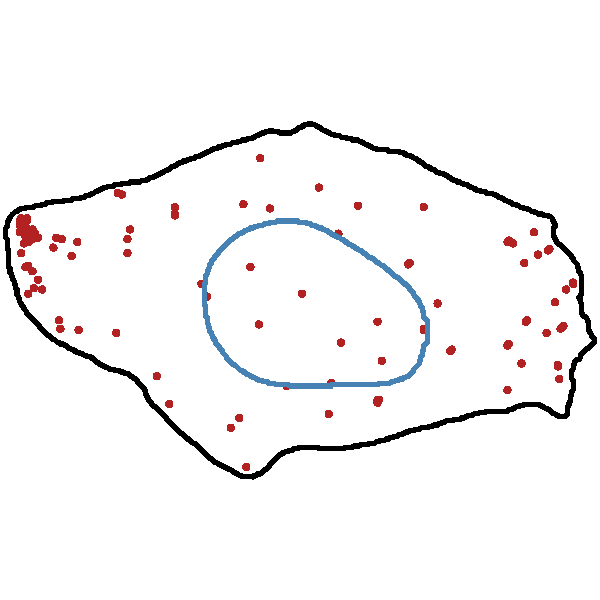
\includegraphics[width=\linewidth]{figures/introduction/real_coord_protrusion}
		\subcaption{Protrusion}
	\endminipage
	\caption[Coordinate representations for different RNA localization patterns]{RNA localization patterns from~\cite{CHOUAIB_2020}.
	Coordinate representations with RNA spots (\textit{red}), cell membrane (\textit{black}) and nuclear membrane (\textit{blue}).
	Detection and segmentation results are extracted and visualized with \emph{bigfish}}
	\label{fig:localization_patterns_racha_features}
\end{figure}

\subsection{PointFISH}
\label{subsec:pointfish}

\subsubsection{Input preparation}

Besides the original \ac{RNA} point cloud, I can use an optional second input vector with my model.
Let $X \in \mathbb{R}^{N \times 3}$ be the original input point cloud with $N$ the number of \ac{RNA}s.
I define my second input vector as $\tilde{X} \in \mathbb{R}^{N \times d}$ with $d \in \{1, 2, 3, 4, 5\}$.
The latter is composed of three contextual inputs.
First I can integrate morphological information by merging \ac{RNA} point cloud with 2D coordinates from the cell and the nucleus membranes.
Such coordinates are localized to the average height of the \ac{RNA} point cloud (0 if it is centered).
This morphological input substantially increases the size of the original point cloud, because I subsample 300 nodes from the cell membrane and 100 nodes from the nucleus one.
I also define an extra boolean vector to indicate the cell nodes and a second one to label the nucleus nodes.
By construction, each \ac{RNA} in the point cloud has then two \emph{False} values.
I end up with $X \in \mathbb{R}^{\tilde{N} \times 3}$ (with $\tilde{N} = N + 300 + 100$) and $\tilde{X} \in \{0, 1\}^{\tilde{N} \times 2}$ as inputs.
Second, I can compute the distance from cell and nucleus for every \ac{RNA} node.
This adds an extra input $\tilde{X} \in \mathbb{R}^{N \times 2}$.
Third, I can leverage the cluster detection algorithm from \emph{bigfish} in order to label each \ac{RNA} node as clustered or not.
It gives us a boolean $\tilde{X} \in \{0, 1\}^{N \times 1}$ to indicate if a RNA belongs to a RNA cluster of not.
Depending on whether or not I choose to add the morphological, the clustering or the distance information, I can exploit up to 5 additional dimensions of input.

\subsubsection{Model architecture}

I adopt the generic architecture introduced by PointNet~\cite{Qi_2017_CVPR}: successive point-wise representations with increasing depth followed by a max pooling operation to keep the network invariant by input permutation.
I incorporate state-of-the-art modules to learn efficient local structures within the point cloud.
As illustrated in Figure~\ref{fig:PointFISH_architecture}, I also adapt the network to the specificity of RNA point clouds.

\begin{figure}[]
    \centering
    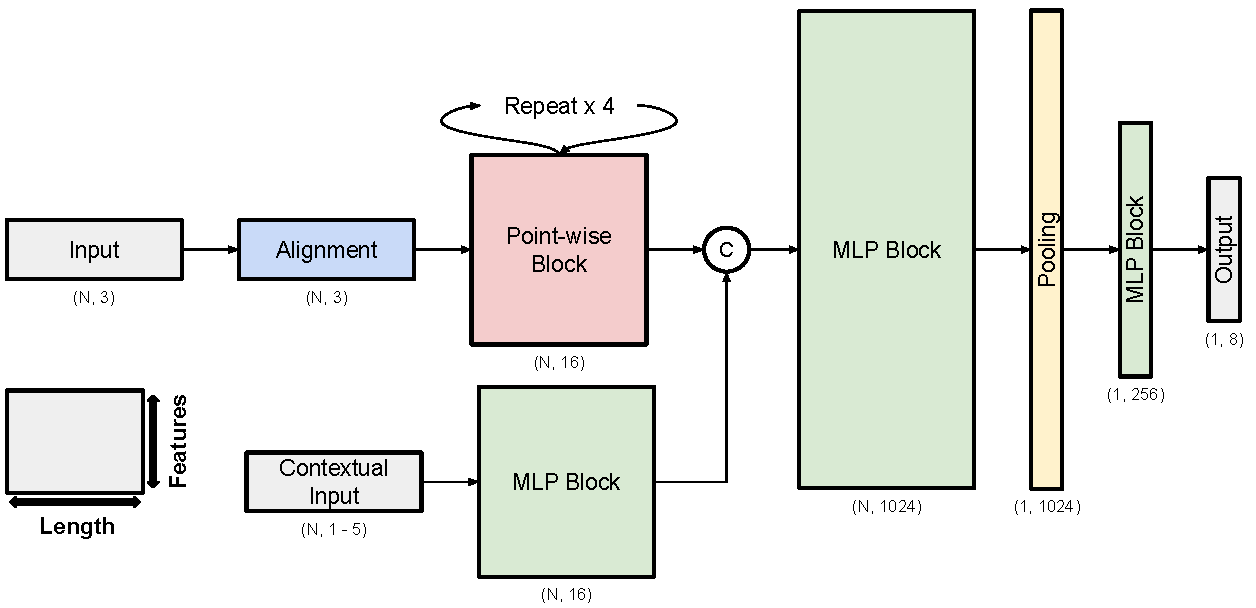
\includegraphics[width=1\textwidth]{figures/chapter4/PointFISH_architecture}
    \caption[PointFISH model]{PointFISH architecture, from~\cite{pointfish_2022}.
	Width and height of \textit{boxes} represent output length and dimension, respectively.
	\textit{Tuples} represent output shapes}
    \label{fig:PointFISH_architecture}
\end{figure}

\paragraph{Point-wise Block}

Instead of shared MLPs like PointNet, I implement a multi-head attention layer based on point transformer layer~\cite{Zhao_2021_ICCV}.
First, I assign to each datapoint $x_i$ its 20 nearest neighbors $X(i) \subset X$, based on the euclidean distance in the features space.
I also compute a position encoding $\delta_{ij} = \theta(x_i - x_j)$ for every pair within these neighborhoods, with $\theta$ a MLP.
Three sets of point-wise features are computed for each datapoint, with shared linear projections $\phi$, $\psi$ and $\alpha$.
Relative weights between datapoints $\gamma(\phi(x_i) - \psi(x_j))$ are computed with the subtraction relation (instead of dot product as in the seminal attention paper~\cite{NIPS2017_3f5ee243}) and a MLP $\gamma$.
These attention weights are then normalized by softmax operation $\rho$.
Eventually, datapoint's feature $y_i$ is computed as weighted sum of neighbors value $\alpha(x_j)$, weighted by attention.
With the position encoding added to both the attention weights and the feature value, the entire layer can be summarized such that:

\begin{equation}
	{\displaystyle y_i = \sum_{x_j \in X(i)} \rho(\gamma(\phi(x_i) - \psi(x_j) + \delta_{ij})) \odot (\alpha(x_j) + \delta_{ij})}
\end{equation}

For a multi-head attention layer, process is repeated in parallel with independent layers, before a last linear projection merges multi-head outputs.
A shortcut connexion and a layer normalization~\cite{ba2016layer} define the final output of my multi-head attention layer.

\paragraph{Alignment Module}

Albeit optional, this module is critical.
Some papers stress the necessity to preprocess the input point cloud by learning a projection to \emph{align} the input coordinates in the right space~\cite{Qi_2017_CVPR,Wang_2019}.
In addition, density heterogeneity across the point cloud and irregular local geometric structures might require local normalization.
To this end, I reuse the geometric affine module described in PointMLP~\cite{ma2022rethinking} which transforms local datapoints to a normal distribution.
With $\{x_{i, j}\}_{j=1,\dots,20} \in \mathbb{R}^{20 \times 3}$, the neighborhood's features of $x_i$, I compute:

\begin{equation}
	{\displaystyle \{x_{i, j}\} = \alpha \odot \frac{\{x_{i, j}\} - x_i}{\sigma + \epsilon} + \beta}
\end{equation}

\noindent
Where $\alpha \in \mathbb{R}^3$ and $\beta \in \mathbb{R}^3$ are learnable parameters, $\sigma$ is the feature deviation across all local neighborhoods and $\epsilon$ is a small number for numerical stability.

\paragraph{Contextual Inputs}

My \ac{RNA} point cloud does not include all the necessary information for a localization pattern classification.
Especially, I missed morphological information.
To this end, deep learning architectures allow flexible insertions.
Several contextual inputs $\tilde{X}$ can feed the network through a parallel branch, before concatenating \ac{RNA} and contextual point-wise features.
My best model exploits cluster and distance information in addition to \ac{RNA} coordinates.

\subsection{Experiment}
\label{subsec:experiment}

\subsubsection{Training and evaluation on simulated patterns}

I train PointFISH on the simulated dataset.
My implementation is based on TensorFlow~\cite{tensorflow_2015}.
I use Adam optimizer~\cite{Diederik_2015} with a learning rate from 0.001 to 0.00001 and an exponential decay (decay rate of 0.5 every 20,000 steps).
Model is trained for a maximum of 150 epochs, with a batch size of 32, but early stopping criterion is implemented if validation loss does not decrease after 10 consecutive epochs.
Usually model converges after 50 epochs.
I apply a 10\% dropout for the last layer and classifications are evaluated with a categorical cross entropy loss.
Even if localization patterns are not necessarily exclusive, for the simulations I trained the model to predict only one pattern per cell.
For this reason, I did not simulate mixed patterns and assume it could help the model to learn disentangled representations.
Training takes 6 to 8 hours to converge with a Tesla P100 GPU.

A first evaluation can be performed on the simulated test dataset.
Because each pattern is equally generated, a simple accuracy metric is enough.
On experimental dataset, imbalanced between localization patterns implies a more robust metric like F1-score.
With my best PointFISH models, I obtain a general F1-score of 95\% over the different patterns (see confusion matrix~\ref{fig:confusion_matrix}).

\begin{figure}[]
    \centering
    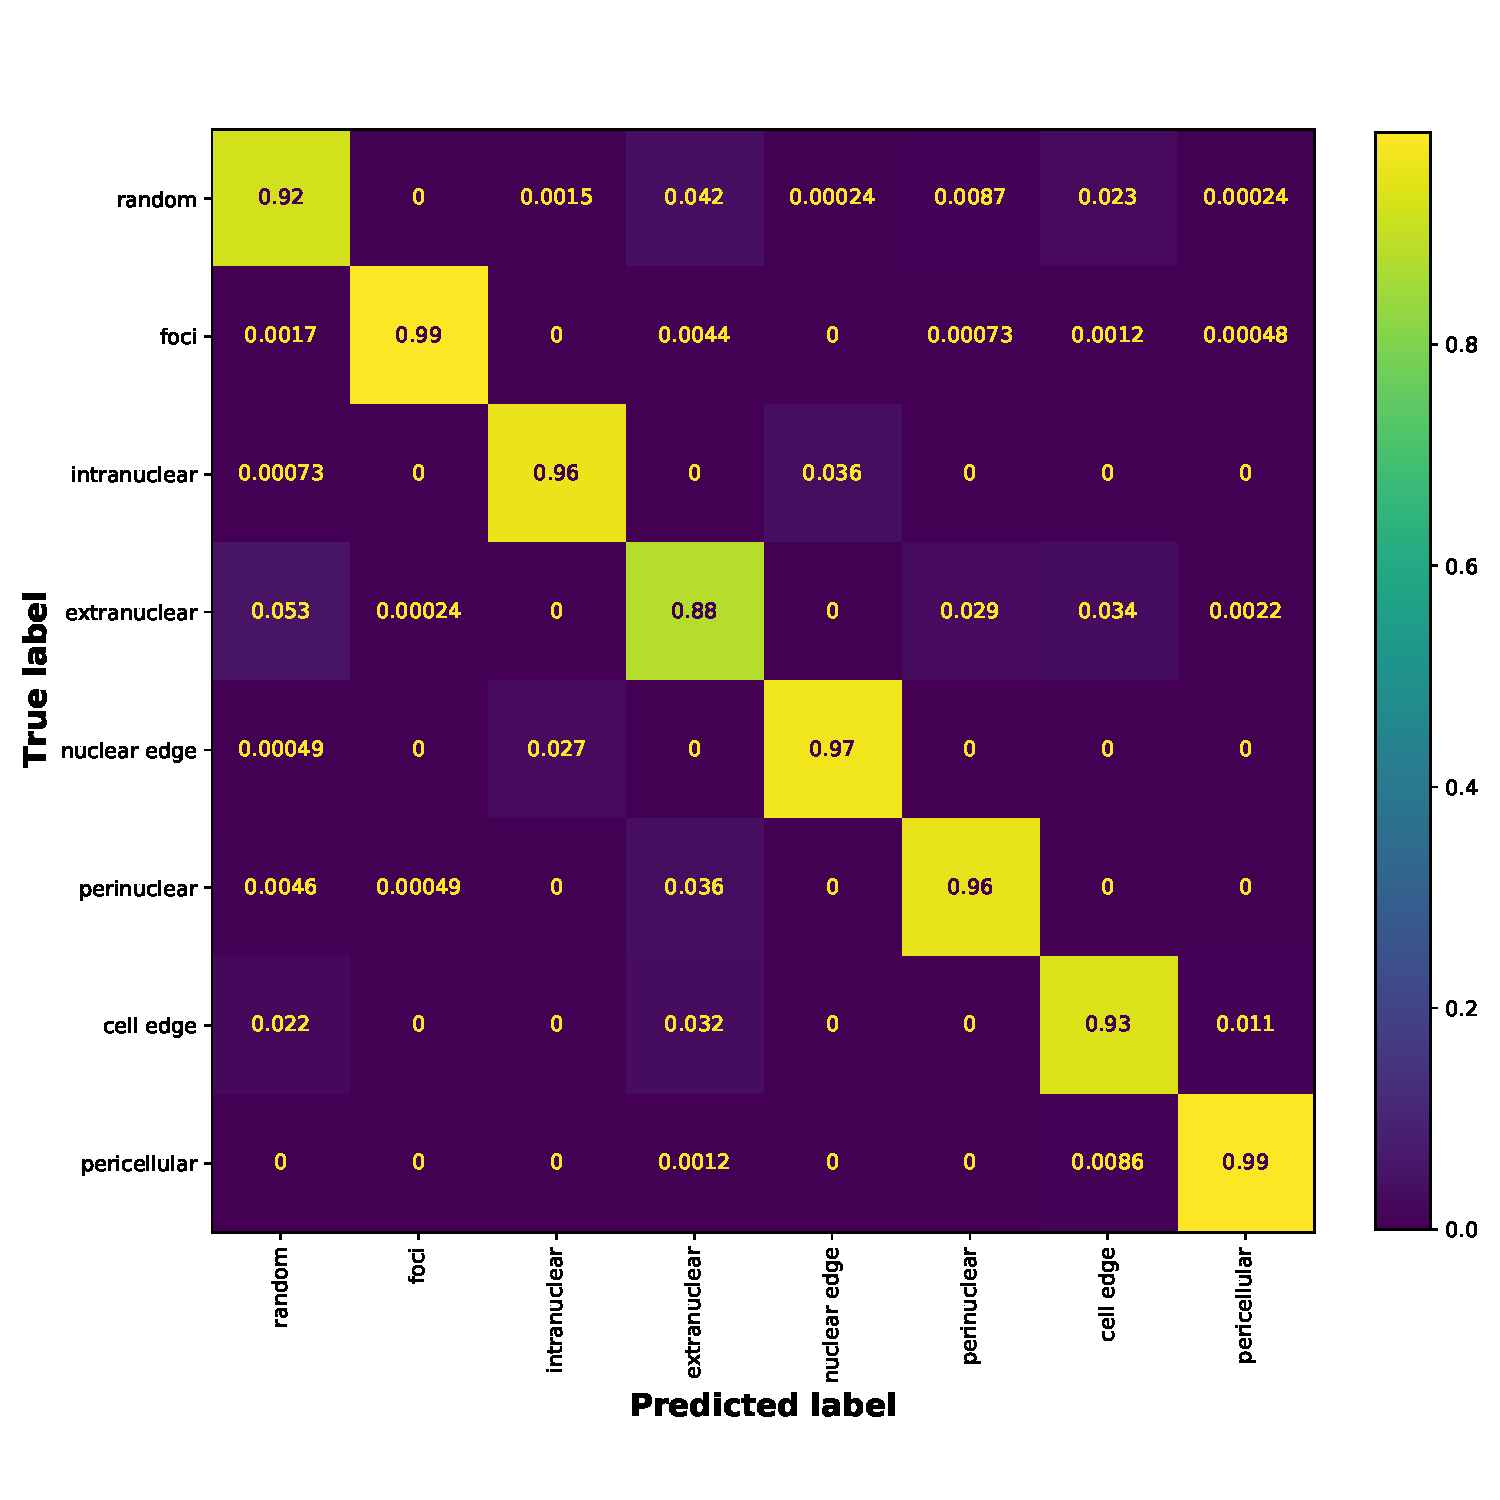
\includegraphics[width=0.7\textwidth]{figures/chapter4/confusion_matrix}
    \caption[Confusion matrix with simulated test set]{Confusion matrix with simulated test patterns (normalized over the \textit{rows})}
    \label{fig:confusion_matrix}
\end{figure}

\subsubsection{Embedding extraction}

From a trained PointFISH model I can remove the output layer to get a feature extractor that computes a 256-long embedding from a \ac{RNA} point cloud.

\paragraph{Learned embedding}

I compute the embedding for the entire cell population studied in~\cite{CHOUAIB_2020}.
All the 9170 cells can be visualized in 2D using a UMAP projection~\cite{McInnes2018}.
In Figure~\ref{fig:umap_real} every point represents a cell.
Among the 810 annotated cells, those with a unique pattern are colored according to the localization pattern observed in their \ac{RNA} point cloud.
The rest of the dataset remains gray.
Overall, PointFISH embedding discriminates well the different localization patterns.
Intranuclear, nuclear edge and perinuclear cells form distinct clusters, despite their spatial overlap, as well as protrusions.
Cells with foci can be found in a separated clusters as well, but also mix with nuclear and perinuclear patterns.
This confusion is not surprising as a large number of cells in the dataset present a nuclear-related foci pattern: cells have \ac{RNA}s clustered in foci, which in turn are close to the nuclear envelope, in which case the cell would be labeled with both patterns.

\begin{figure}[]
    \centering
    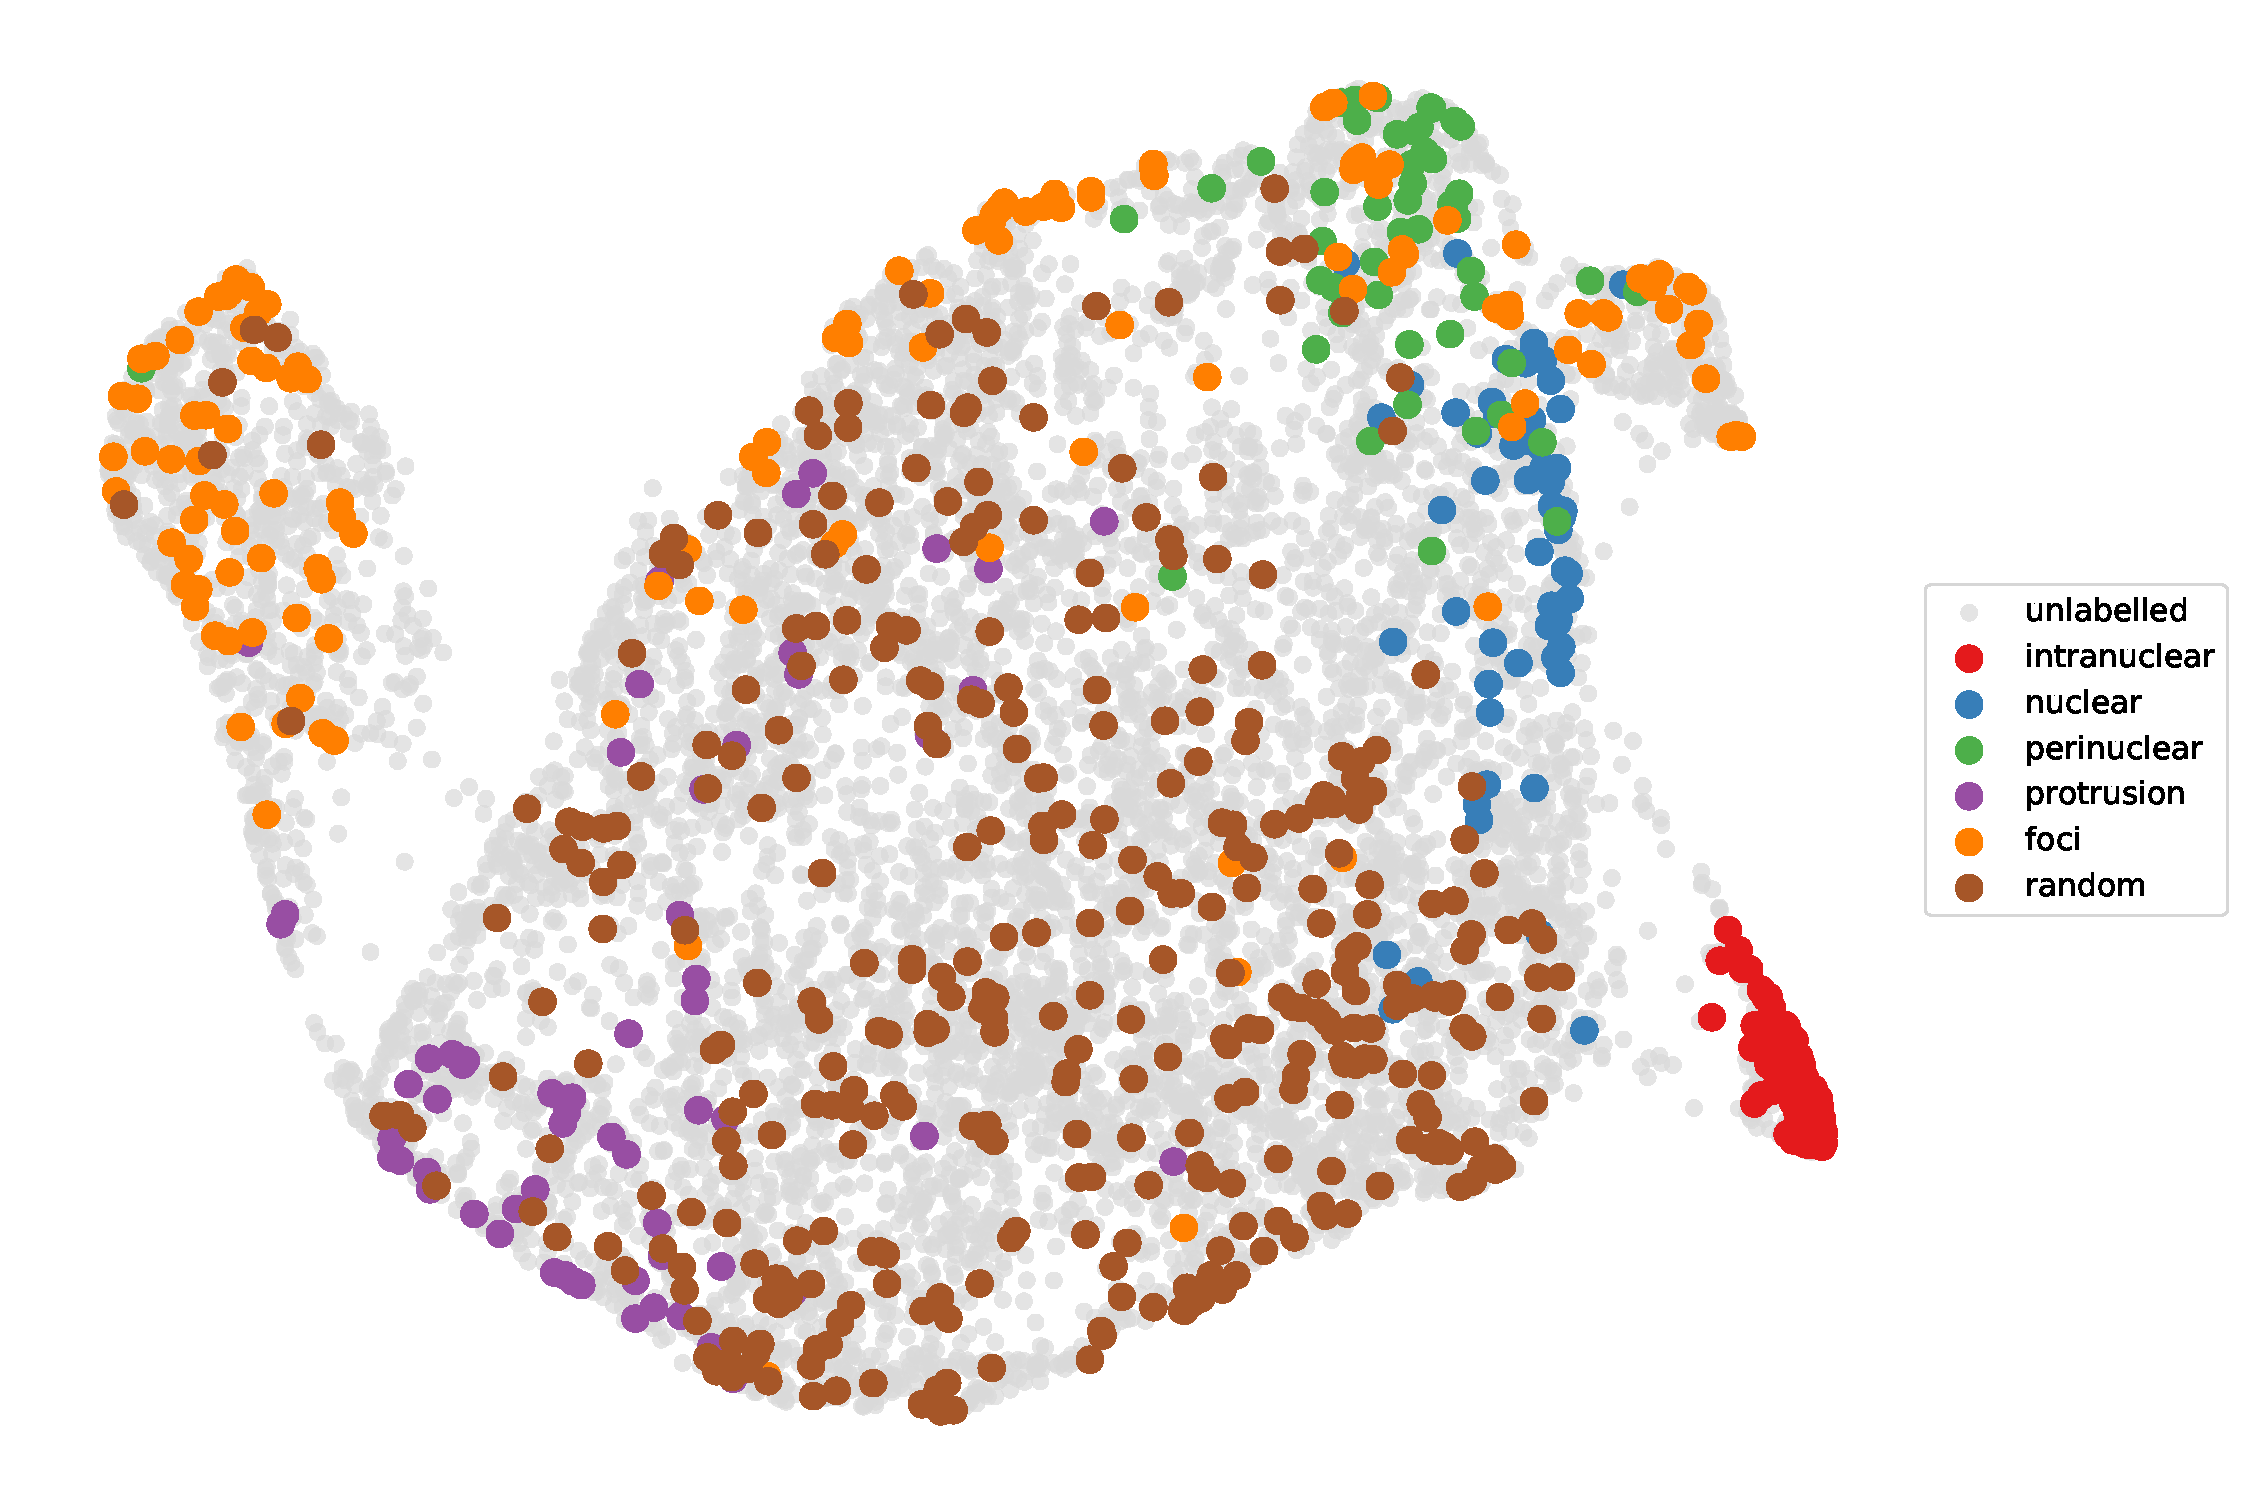
\includegraphics[width=\textwidth]{figures/chapter4/umap_real}
    \caption[UMAP embedding with exprimental dataset]{UMAP embedding with learned features, from~\cite{pointfish_2022}.
	Each point is a cell from experimental dataset.
	Manually annotated cells are colored according to their localization pattern}
    \label{fig:umap_real}
\end{figure}

\paragraph{Supervised classification}

Because PointFISH already return meaningful embeddings, I can apply a simple classifier on top of these features to learn localization patterns.
I use the 810 manually annotated cells from the experimental dataset.
I compare the 15 hand-crafted features selected in~\cite{CHOUAIB_2020} with my learned embedding.
Every set of features is rescaled before feeding a classifier.
Expert features include:

\begin{itemize}
	\setlength\itemsep{0.1em}
	\item The number of foci and the proportion of clustered \ac{RNA}s.
	\item The average foci distance from nucleus and cell (normalized by the expected distance with a random foci distribution).
	\item The proportion or \ac{RNA}s inside nucleus.
	\item The average \ac{RNA} distance from nucleus and cell (normalized by the expected distance with a random \ac{RNA} distribution).
	\item The number of \ac{RNA}s detected in cell extensions (normalized by the expected number with a random \ac{RNA} distribution) and the peripheral dispersion index~\cite{stueland_rdi_2019}.
	\item The number of \ac{RNA}s within different relevant subcellular regions (normalized by the expected number with a random \ac{RNA} distribution).
\end{itemize}

\begin{figure}[]
    \centering
	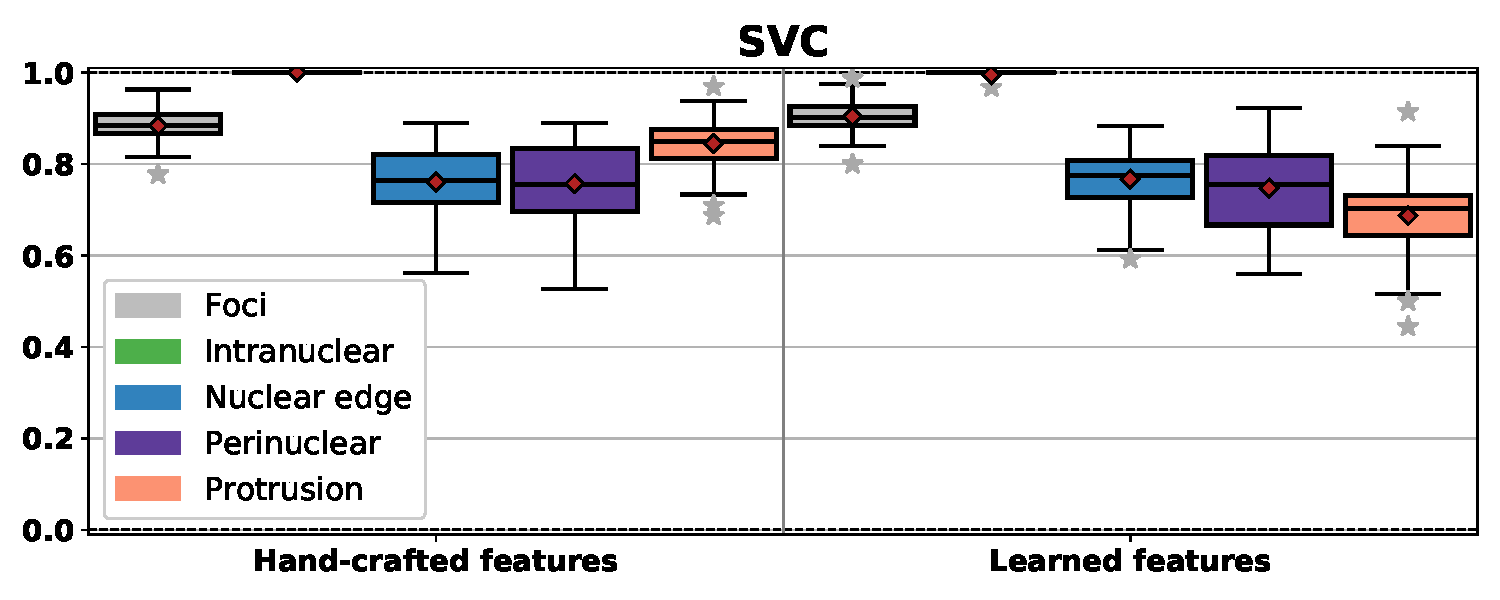
\includegraphics[clip, trim=0cm 0cm 0cm 1cm, width=\textwidth]{figures/chapter4/f1_SVC}
    \caption[F1-score distribution with hand-crafted and learned features]{F1-score distribution of localization pattern classification (SVC model), from~\cite{pointfish_2022}}
    \label{fig:f1_SVC_real}
\end{figure}

I design 5 binary classification tasks, one per localized pattern (random pattern is omitted).
The classifier is a SVC model~\cite{chang2011libsvm}.
For evaluation purpose, I apply a nested cross-validation scheme.
First a test set is sampled from the dataset (20\%), then the remaining cells are used with a gridsearch to fit an optimal SVC model (with a 20\% validation split).
Parameters grid includes the choice between a linear or a RBF kernel and the strength of the regularization.
The entire process is repeated 50 times, with different test split, and F1-score for each classification task is returned.
This full evaluation pipeline is implemented with \emph{scikit-learn}~\cite{scikit-learn}.
F1-score's distribution over 50 splits are summarized in Figure~\ref{fig:f1_SVC_real}.
Learned features match performances of hand-crafted features selected for the tasks.
While the recognition of localization in protrusions is slightly worse, it is important to point out that I did not include simulations of this patterns in the training dataset.

\subsubsection{Ablation study}

I perform several ablation studies to evaluate the impact of different components in PointFISH model.
In the point cloud literature, papers often propose new modules to improve network's performances, but they implement them in slightly different architectures.
Heterogeneity in terms of normalization, latent dimensions or layer size complicate comparisons between techniques.
In order to isolate the importance of each element, I use a template architecture as illustrated in Figure~\ref{fig:PointFISH_architecture}.
Instead of comparing PointFISH with DGCNN, I compare PointFISH with an equivalent networks where attention layers are replaced by EdgeConv~\cite{Wang_2019}.
The rest of the network remains strictly identical.

\paragraph{Additional input}

\begin{wraptable}{R}{0.60\textwidth}
	\centering
	\begin{tabular}{| c | c | c | c |}
		\hline
		Distance & Cluster & Morphology & F1-score \\
		\hline
		\ding{55} & \ding{55} & \ding{55} & 0.42\\
		\checkmark & \ding{55} & \ding{55} & 0.74\\
		\ding{55} & \checkmark & \ding{55} & 0.45\\
		\checkmark & \checkmark & \ding{55} & $0.81^{\ast}$\\
		\checkmark & \checkmark & \checkmark & \textbf{0.82}\\
		\hline
	\end{tabular}
	\caption[Impact of contextual inputs (PointFISH)]{Impact of contextual inputs, from~\cite{pointfish_2022}.
	F1-score is averaged over 4 trainings with different random seeds.
	Best model is in bold.
	Reference model is labelled with $\ast$}
	\label{table:extra_inputs}
\end{wraptable}

I compare the use of \ac{RNA} point cloud only as input or the inclusion of contextual inputs through a parallel branch.
\ac{RNA} coordinates do not have any morphological information about the cell.
In Table~\ref{table:extra_inputs}, this design logically returns the lowest F1-score.
Three additional inputs are available: \ac{RNA} distance from cell and nucleus (\emph{distance}), \ac{RNA} clustering flag (\emph{cluster}) and the integration of cell and nucleus membrane coordinates (\emph{morphology}).
Best performances are obtained with, at least, distance and cluster information.
Cell and nucleus coordinates do not increase significantly the classification and dramatically increase the computation time of the model (I need to process a larger point cloud).
In particular, cluster information greatly improves foci pattern recognition while distances boost others localization patterns.

\paragraph{Alignment module and Point-wise block}

To measure the impact of the geometric affine module~\cite{ma2022rethinking} I compare it with the TNet module implemented in PointNet~\cite{Qi_2017_CVPR}.
I also design a variant TNetEdge where MLP layers extracting point-wise independent features are replaced with EdgeConv layers.
Results are reported in Table~\ref{table:ablation}.
An alignment block seems critical at the beginning of the network.
However, the geometric affine module is both more efficient (F1-score of 0.81) and much lighter than TNet and TNetEdge.

From the PointNet and DGCNN seminal articles, I also compare the use of their respective point-wise blocks against my multi-head attention layer.
As expected, EdgeConv blocks convey a better information than PointNet by exploiting local neighborhood within point cloud (F1-score of 0.78 and 0.75 respectively).
Yet, they do not match the performance of multi-head attention layer.

Concerning these layers, I evaluate how the number of parallel heads can influence the performance of PointFISH.
By default, I use 3 parallel attention layers to let the model specialized its attentions vectors, but I also test 1, 6 and 9 parallel heads.
In Table~\ref{table:ablation} we only observe a slight benefit between the original point transformer layer~\cite{Zhao_2021_ICCV} (without one attention layer) and its augmented implementation.

% multiscale
% k neigbors

\paragraph{Latent dimensions}

The second part of PointFISH architecture is standardized: a first MLP block, a max pooling operation, a second MLP block and the output layer.
I quantify the impact of additional MLP layers within these blocks.
My reference model returns an embedding with 256 dimensions (before the output layer).
In a MLP block, I use ReLU activation and layer normalization, but also increase or decrease the depth by a factor 2 between layers.
Before the pooling layer, the first MLP block includes 4 layers with an increasing depth (128, 256, 512 and 1024).
After the pooling layer, the second MLP block includes 2 layers with a decreasing depth (512 and 256).
Similarly, to return 128, 64 or 32 long embeddings, I implement 6 (128, 256, 512, pooling, 256 and 128), 5 (128, 256, pooling, 128 and 64) or 4 final layers (128, pooling, 64 and 32).
We observe in Table~\ref{table:ablation} a fall in performance for the lowest dimensional embedding (64 and 32).
This hyperparameter is also critical to design lighter models, with a division by 4 in terms of trainable parameters between a 256 and a 128 long embedding.

\begin{table}[]
	\centering
	\begin{tabular}{| c | c | c | c | c | c |}
		\hline
		Alignment & Point-wise block & \# heads & \# dimensions & \# parameters & F1-score \\
		\hline\hline
		- & Attention layer & 3 & 256 & 1,372,608 & 0.73\\
		TNet & Attention layer & 3 & 256 & 1,712,521 & 0.74\\
		TNetEdge & Attention layer & 3 & 256 & 1,589,321 & 0.74\\
		\hline\hline
		Affine & MLP & - & 256 & 1,374,526 & 0.75\\
		Affine & EdgeConv & - & 256 & 1,387,006 & 0.78\\
		\hline\hline
		Affine & Attention layer & 9 & 256 & 1,403,334 & \textbf{0.82}\\
		Affine & Attention layer & 6 & 256 & 1,387,974 & \textbf{0.82}\\
		Affine & Attention layer & 3 & 256 & 1,372,614 & $0.81^{\ast}$\\
		Affine & Attention layer & 1 & 256 & 1,362,374 & 0.81\\
		\hline\hline
		Affine & Attention layer & 3 & 128 & 352,966 & 0.81\\
		Affine & Attention layer & 3 & 64 & 97,094 & 0.77\\
		Affine & Attention layer & 3 & 32 & 32,646 & 0.75\\
		\hline
	\end{tabular}
	\caption[Ablation studies (PointFISH)]{Ablation studies on experimental dataset, from~\cite{pointfish_2022}.
	F1-score is averaged over 4 trainings with different random seeds.
	Best models are bold.
	Reference model is labelled with $\ast$}
	\label{table:ablation}
\end{table}

\subsection{Discussion}
\label{subsec:discussion}

Being able to directly process list of points provides the community with a tool to integrate large datasets obtained with very different techniques on different model systems.
While the actual image data might look strikingly different between such projects, they can all be summarized by segmentation masks of nuclei and cytoplasm, and a list of coordinates of \ac{RNA} locations.
Besides being a straightforward approach, having methods that act directly on point clouds is also a strategic advantage.

The idea of training on simulated data provides us the opportunity to query datasets with respect to new localization patterns that have not yet been observed, and for which I do not have real examples so far.
In addition, this strategy allows us to control for potential confounders, such as cell morphology, or number of \ac{RNA}s.

I finally provide a generic method that can leverage these simulations, without the tedious process of handcrafting new features.
It is not necessary that the simulated patterns are optimized as to resemble real data.
They rather serve as a pretext task.
If a network is capable of distinguishing the simulated patterns, chances are high that the corresponding representation is also informative for slightly or entirely different patterns.
Likewise, representations trained on ImageNet can be used for tumor detection in pathology images.
I show this by omitting the protrusion pattern from the simulation.
Indeed, in Figure~\ref{fig:umap_real}, the protrusion patterns live in a particular region of the feature space, without specific training.

% reference ImageNet
% reference tumor detection in pathology images

As a future work, a first valuable task would be the development or the sourcing of annotated datasets with various cell lines and imaging conditions.
The difficulty of gathering experimental training datasets can be overcome by simulations.
However, I still need to extend my evaluation across different benchmarks to assess the robustness of a point cloud model.
Among the examples of interest, recent publications~\cite{savulescu_interrogating_2021,mah_bento_2022} evaluate their methods on their own datasets, which include \ac{RNA} localization annotations.
Second, a better engineering of PointFISH could make contextual inputs irrelevant and only base predictions on the point cloud coordinates.
A third potential improvement concerns the segmentation.
I exploit so far a 2D segmentation because it is the more frequent usecase and the task for which I have a large number of trained models available.
Yet, a 3D segmentation mask would allow a more complete 3D point cloud mixing \ac{RNA} and cell datapoints.
This could also dramatically improve pattern representation.
Last but not least, training a point cloud model with a self-supervised training procedure would result in task-independent representations.
This could eventually help to generalize over unknown localization patterns.

\section{Conclusion}
\label{sec:analysis_conclusion}

I first present the coordinate representation of the cell, from which I base my feature engineering and my statistical analysis.
On the top of existing solutions to extract \ac{RNA} spots and cell morphology coordinates, I then list the different hand-crafted features I designed to quantify and classify \ac{RNA} localization patterns.
These features are implemented in \emph{bigfish.classification}.
Lastly, in the third section, I propose to directly process the extracted point clouds, without the need to design handcrafted features.
For this, I leverage coordinates of simulated localization patterns to train a specifically designed neural network taking as input a list of points and associated features that greatly enhance generalization capabilities.
Recent advances in point cloud analysis through deep learning models allows us to build a flexible and scalable pipeline that fits with \ac{RNA} point cloud specificity.
I show that this method is on par with carefully designed, handcrafted feature sets.

% learned features from convnet
% from features engineering to simulation engineering
% limitations